\chapter{Code for calculating synchrotron radiation in a waveguide}
\label{chapter:Synchrotron_radiation_in_a_wave_guide}

\rr{correct the intro where it's not actual with what was presented}
\rr{all citations will be included later (I have all them in mind, but inserting them is a bit tedious and distracting from writing)}
\rr{probably add the name of the code SRinWG of SRinWaveGuide}
    
    Generation of synchrotron radiation is typically considered in free space, where the problem adheres to a natural boundary condition: the field diminishes to zero at infinity. This assumption serves as a practical approximation since, even though at the real facilities radiation is generated and propagates within vacuum pipes and faces another components like mirrors, apertures, flanges, detectors etc, their influence on radiation in a wide range of wavelengths (from visible light up hard X-ray and higher) is often negligible to an undetectable level. However, when dealing, for instance, with THz radiation it becomes necessary to consider the effects of these metallic components on the radiation, especially the vacuum pipes. In this chapter, I introduce a numerical code that is designed to calculate synchrotron radiation in the presence of boundary conditions of perfectly conducting metallic walls… \rr{say that the walls are considered to be perfectly conducting and what would be the result with normal medium}
    
    Theoretical background for this problem was founded in~\rr{cite}, that extends and complement prior works~\rr{cite}. The goal of this work is to develop a code based on derivation made in~\rr{cite} capable of accurately calculating synchrotron radiation accounting for the waveguide effects, e.g. imposed by the metallic components of the beamlines. This is essential for the precise numerical simulation of the performance of insertion devices at THz beamlines. Such a tool is crucial for designing THz radiation propagation lines at facilities, including those planned or under construction at SLAC~\rr{cite} and the European XFEL~\rr{cite}, as well as those had been already in operational e.g. FLASH, \rr{is there more}. The method I employed to program a code utilizes the Green's function approach to solve the field equation. This approach offers considerable flexibility; once the Green's function for a given system is determined—which can be usually analytically derived for simple, yet practical geometries—one only needs to take an integral over the right-hand side of the wave equation. The right-hand contain an electron trajectory and velocity that can easily can be found analytically or solving this numerically with tools like those~\rr{cite}
    
    Within this chapter, I deduce the boundary conditions for a waveguide with an arbitrary cross-section, present the general form of the integral that is to be taken, and provide the expression for the Green's function for an axially symmetrical metallic waveguide based on~\rr{cite}. A significant part of this chapter is dedicated to cross-validating the developed code. The verification process begins with a straightforward scenario of synchrotron radiation in free space using corresponding Green's function of the Helmholtz equation. This step is done to cross-check the integration process itself. The results of the developed code I cross-check with Synchrotron Radiation Workshop (SRW)~\rr{cite}. Only then I cross-validate the results obtained with the Green's function of a circular waveguide. I test the results in the limit of free space: I take the waveguide Green's function, increase the tube's radius ($R$), and compare these results with those obtained using the free space Green's function. Finally, in a real scenario where there is a strong influence of the walls for a ten-period undulator device, I cross-check the results of the code with analytical expressions.
    
    The developed code has been uploaded to a GitHub repository~\rr{cite}, with plans for further development to meet the demands of accurate THz radiation beamline simulations. The development and cross-checks of the code have revealed several challenges that necessitate further studies. For instance, the Green's function of the bounded system is an infinite sum of transverse modes, and identifying which of these modes effectively contribute to the integral beforehand is crucial: some modes lead to the appearance of highly oscillatory integrals, which result in aliasing issues, while their contributions are negligible. Additionally, enhancements are needed in the code's numerical efficiency, along with addressing other programming-related issues in potential future work.
    
\section{Boundary conditions}
    
    In Chapter~\ref{chapter:Synchrotron radiation}, I considered the solution of the wave equation for a single electron moving on an arbitrary trajectory in free space within the paraxial approximation. This treatment will now be extended to the case of a single electron moving in a magnetic field in the presence of \rr{perfectly conducting} metallic boundaries. Before deriving formulas and accounting for the boundary conditions, one must assume that the waveguide is overmoded for the given wavelength, e.g., $\lambdabar \ll R$, following~\rr{cite}, to ensure that the slowly varying envelope approximation can be applied. Additionally, one needs to confirm the applicability of the paraxial approximation in the presence of a waveguide, which generally holds when $k_{\perp}^2 c^2 / \omega^2 \ll 1$, where $k_{\perp}$ is the transverse wave number. To extend this to the case with the waveguide, this condition should also hold for each mode in the waveguide.
    
    For the metallic walls boundary conditions means that the electric field must be perpendicular to the surface ($S$).
        \begin{align}
            \left(n_x \widetilde{E}_y - n_y \widetilde{E}_x\right)_{\big|_S}=
            \left(\vec{n} \times \vec{\widetilde{E}}_\bot\right)_{\big|_S} = 0
        \end{align}
    and 
        \begin{align}
            \left(\widetilde{E}_{z}\right)_{\big|_S}= 0.
        \end{align}
    One of the Maxwell's equation for the curl of the magnetic field can be written as the following:
        \begin{align}
            \left[\left(\vec{\nabla} \times \vec{\widetilde{H}} \right)_{z}\right]_{\big|_{S}}= 0. 
        \end{align}
    And in the paraxial approximation we make use of the relation for the magnetic field and electric: $\widetilde{E}_x \simeq \widetilde{H}_y$ and $\widetilde{E}_y \simeq -\widetilde{H}_x$. Having both of the conditions: on the amplitude of the field and on its derivatives I write:
        \begin{align}
            \left(\frac{\partial \widetilde{E}_x}{\partial x} + \frac{\partial
            \widetilde{E}_y}{\partial y}\right)_{\big|_{S}} =
            \left(\vec{\nabla}_\bot \cdot
            \vec{\widetilde{E}}_\bot\right)_{\big|_S} = 0
        \end{align}
    So, writing together the wave equation and the boundary condition I obtain the following system:
        \begin{align}
            \left\{
            \begin{array}{l}
            \mathcal{D} \left[\vec{\widetilde{E}}_\bot(z,\vec{r}_\bot)\right]
            = \vec{f}(z, \vec{r}_\bot)
            \\
            \left(\vec{n} \times \vec{\widetilde{E}}_\bot\right)_{\big|_S} = 0
            \\
            \left(\vec{\nabla}_\bot \cdot
            \vec{\widetilde{E}}_\bot\right)_{\big|_S} = 0~,
            \end{array}\right.
            \label{Eq:boundary_conditions}
        \end{align}

    This system should be solved for the given vacuum pipe shape. One can find the solutions for a general case of an arbitrary shape and for the circular waveguide in~\rr{cite}. Once the Green's function is known the slowly carrying envelope of the electron field is written in the following form:
    \begin{align}
        \widetilde{E}^{\alpha}(\vec{r}_\bot,z) = \int_{-\infty}^{z} dz'
        \int d\vec{r'}_\bot~ G^\alpha_\beta\left(\vec{r}_\bot,
        \vec{r'}_\bot,z-z'\right) f^\beta\left(\vec{r'}_\bot,z'\right),
        \label{Eq:field_integral_tensor}
    \end{align}
    or writing it explicitly:
    \begin{align}
        &&\widetilde{E}^\alpha = \frac{4\pi e}{c} \int_{-\infty}^{z} dz'
        \left\{ \frac{i\omega}{c^2} \fcolorbox{black}{blue!30}{$\stackrel{\text{velocity term}}{v_\bot^\beta(z')
        G^\alpha_\beta\left(\vec{r}_\bot,\vec{r'}_\bot(z'), z-z'
        \right)}$}+\fcolorbox{black}{orange!30}{$\stackrel{\text{gradient term}}{\partial'_\beta
        G^\alpha_\beta\left(\vec{r}_\bot,\vec{r'}_\bot(z'), z-z'\right)}$}
        \right\}\cr &&\times \exp\left[\frac{i\omega}{2c} \int_0^{z'}
        \frac{d\bar{z}}{\gamma^2_z(\bar{z})} \right].
        \label{Eq:field_integral_tensor_full}
    \end{align}
    \rr{what is the integration limits for the second integral?}
    The integral contains the Green's function $G^\alpha_\beta$ that is actually not a scalar value but a tensor.

    This integral should be calculated with a given Green's function. As one can see, it is possible to use any Green's function; in this sense, the problem is divided into two steps. First, one needs to derive or calculate a Green's function for a given system, which is basically the solution to the eigenvalue problem for the operator $\mathcal{D}$, including the boundary condition from the system in Eq.~\ref{Eq:boundary_conditions}. Then, take the integral in Eq.~\ref{Eq:field_integral_tensor} that is composed from the right-hand side of the wave equation in Eq.~\ref{Eq:boundary_conditions}. I explicitly take the integral. The uniqueness of this approach is that any Green's function, once known, can be substituted as an input in the code, and the field distribution can be calculated.


\section{Numerical algorithm}
    In this section, I provide detail on the calculation algorithm for taking integral under Eq.~\ref{Eq:field_integral_tensor_full}. For evaluating the field $\widetilde{E}^\alpha$ one need to calculate the integrant expression, which include: taking the integral $\int_0^{z'}
    d\bar{z}/\gamma^2_z(\bar{z})$, calculating the velocity term, and estimating the gradient term. 
    
    Integration for both integrals is performed trivially and can be made with variety of the integration rules: rectangle rule, trapezoidal rule, and more advanced Gauss–Legendre quadrature formula with three points, which provide the accuracy of $\mathcal{O}(h^{1})$, $\mathcal{O}(h^{2})$, and $\mathcal{O}(h^{5})$ with respect to grid spacing, where $\mathcal{O}$ is Big O notation or Bachmann–Landau notation. Simpson's rule with accuracy order of $\mathcal{O}(h^{4})$ shall to be implemented, although I used trapezoidal rule in the following cross-checks being more accurate then trivial rectangle rule and faster then using Gauss–Legendre quadrature formula. For practical applications in numerical simulation this level of accuracy is enough.

  

    As the end goal is to write a code that can accept an arbitrary Green's function taking the derivative should be done numerically following the definition:
        \begin{align}
           f'(x) = \lim_{h \to 0} \frac{f(x + h) - f(x)}{h}, 
           \label{Eq:numerical_derivative}
        \end{align}
    where $x$ is the transverse coordinate variable of a general function $f$ and $h$ is the step along $x$. Taking the derivative numerically requires careful choice of the $h$. For this, I used an adaptive step size formula for the increment $h = \sqrt{\epsilon} x$ or $h = \sqrt{\epsilon}$ if $x = 0$, where $\epsilon$ is machine precision, to avoid rounding errors in case of small $h$ and the errors of differentiation formula itself on the the other side. This insures adequate accuracy of this formula. Interesting, the accuracy of the formula is limited by the estimation of $-f^{(3)}(c) h^2 / 6$, where $c$ is a point in between $x$ and $x + h$. The first order term in canceled naturally due to subtraction operations in Eq.~\ref{Eq:numerical_derivative}. 

    The integration and taking derivative methods can be further improved and also tested, i.e. result of the of different integration rules should be compared, there a formula for five-point method for taking the derivative etc. In the chapter I present the first result on this method and chosen accuracy integration and differentiation is enough for the purpose of cross-checks. The code will be improved at the next iteration of the development.
    
\section{Cross-checks}

    In this section, I will first cross-check the code for the free-space Green's function against the results provided by the Synchrotron Radiation Workshop (SRW) \rr{cite} to ensure the correctness of the chosen approach. It is also essential to examine the 'gradient term,' as the derivative is taken numerically, which may lead to a loss in accuracy and introduce numerical artifacts. Then, I will evaluate the code's performance for the waveguide Green's function. I will verify that the free-space limit is achieved by increasing the radius of the waveguide and subsequently compare it with the analytical expression for undulator radiation in resonance within a waveguide, as described in \rr{cite}.

\subsection{Free space Green's function}

    Typically, codes for calculating synchrotron radiation employ an expression where the free space Green's function is already substituted, and the derivative is taken analytically. Additionally, it is possible to further adjust the integral to prevent the emergence of highly oscillatory contributions, which I will discuss later in the section. This ensures a certain robustness of this approach compared to using the solution of the field equation in its general form with an arbitrary Green's function. The latter requires taking a numerical derivative, which is especially pronounced in the case of edge radiation \rr{cite}. In this instance, the code's limits of applicability should be verified.

    I will present a cross-check of the radiation field calculation results from different magnetic structures with SRW. I will examine a simple arrangement of bending magnets, a three-pole device, an undulator, and one special case, although it is not very possible from a physics perspective. I will discuss several numerical techniques to ensure the physical correctness of the resulting distributions.

\subsubsection{Bending magnet radiation}

    The bending magnet synchrotron radiation drew the attention of researchers at the dawn of synchrotron radiation studies. Despite its apparent simplicity, this source actually has a rigorously complicated structure. Specifically, it concerns the manner in which radiation forms, thereby possessing a nontrivial source structure of single electron (or filament beam) emission. \rr{cite Oleg's paper and GG work}. 
    \begin{figure}[h!]
        \centering
        \begin{subfigure}[c]{0.5\linewidth}
            \centering
            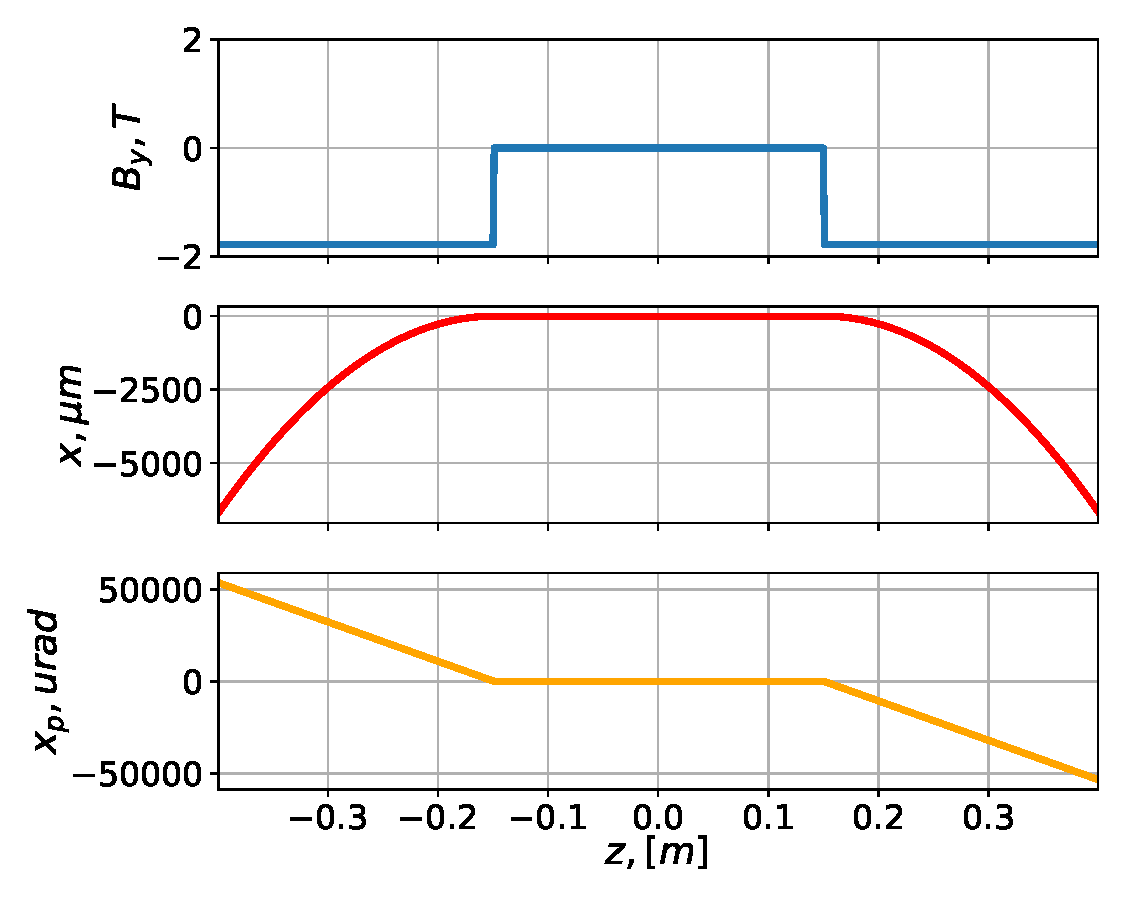
\includegraphics[width=\linewidth]{content/images/5_THz_Source/bend_traj.pdf}
            \caption{From top to bottom: $y$ component of the magnetic field, $x$ component of the trajectory and $x_p$ is the angel of the electron's direction.} % Optional individual caption for the first subfigure
            \label{Fig:bending_traj}
        \end{subfigure}%
        % Add a little space between figures if desired
        \begin{subfigure}[c]{0.5\linewidth}
            \centering
            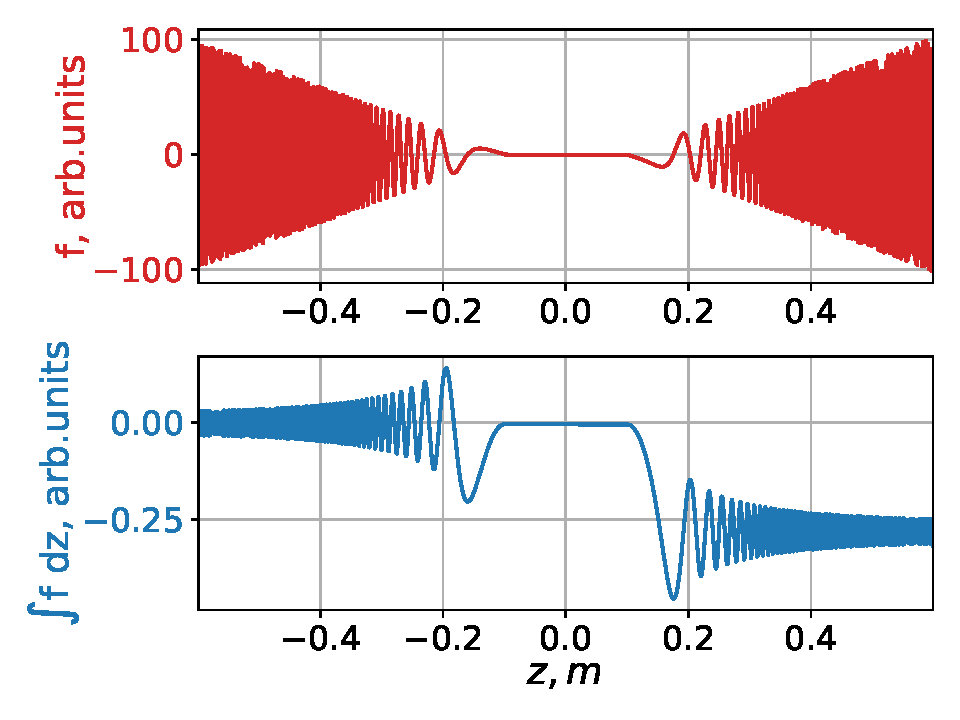
\includegraphics[width=\linewidth]{content/images/5_THz_Source/bend_integral.pdf}
            \caption{Integrant value with respect to $z$ value and corresponding integral value for the bending magnet radiation.} % Optional individual caption for the second subfigure
            \label{Fig:bending_integral}
        \end{subfigure}
        \caption{Bending magnet trajectory and integral evaluation with respect to the longitudinal coordinate.} % Optional overall caption
        \label{Fig:bending_magnet_figs}
    \end{figure}
    Also, radiation from a bending magnet can be non-trivial to calculate numerically, especially in the case of seemingly simple arrangements like the one presented in Fig.~\ref{Fig:bending_traj}. This case is chosen for the sake of cross-checking, as it encompasses all the effects that one must consider when calculating synchrotron radiation. 
    
    \begin{figure*}[h!]
    	\centering
        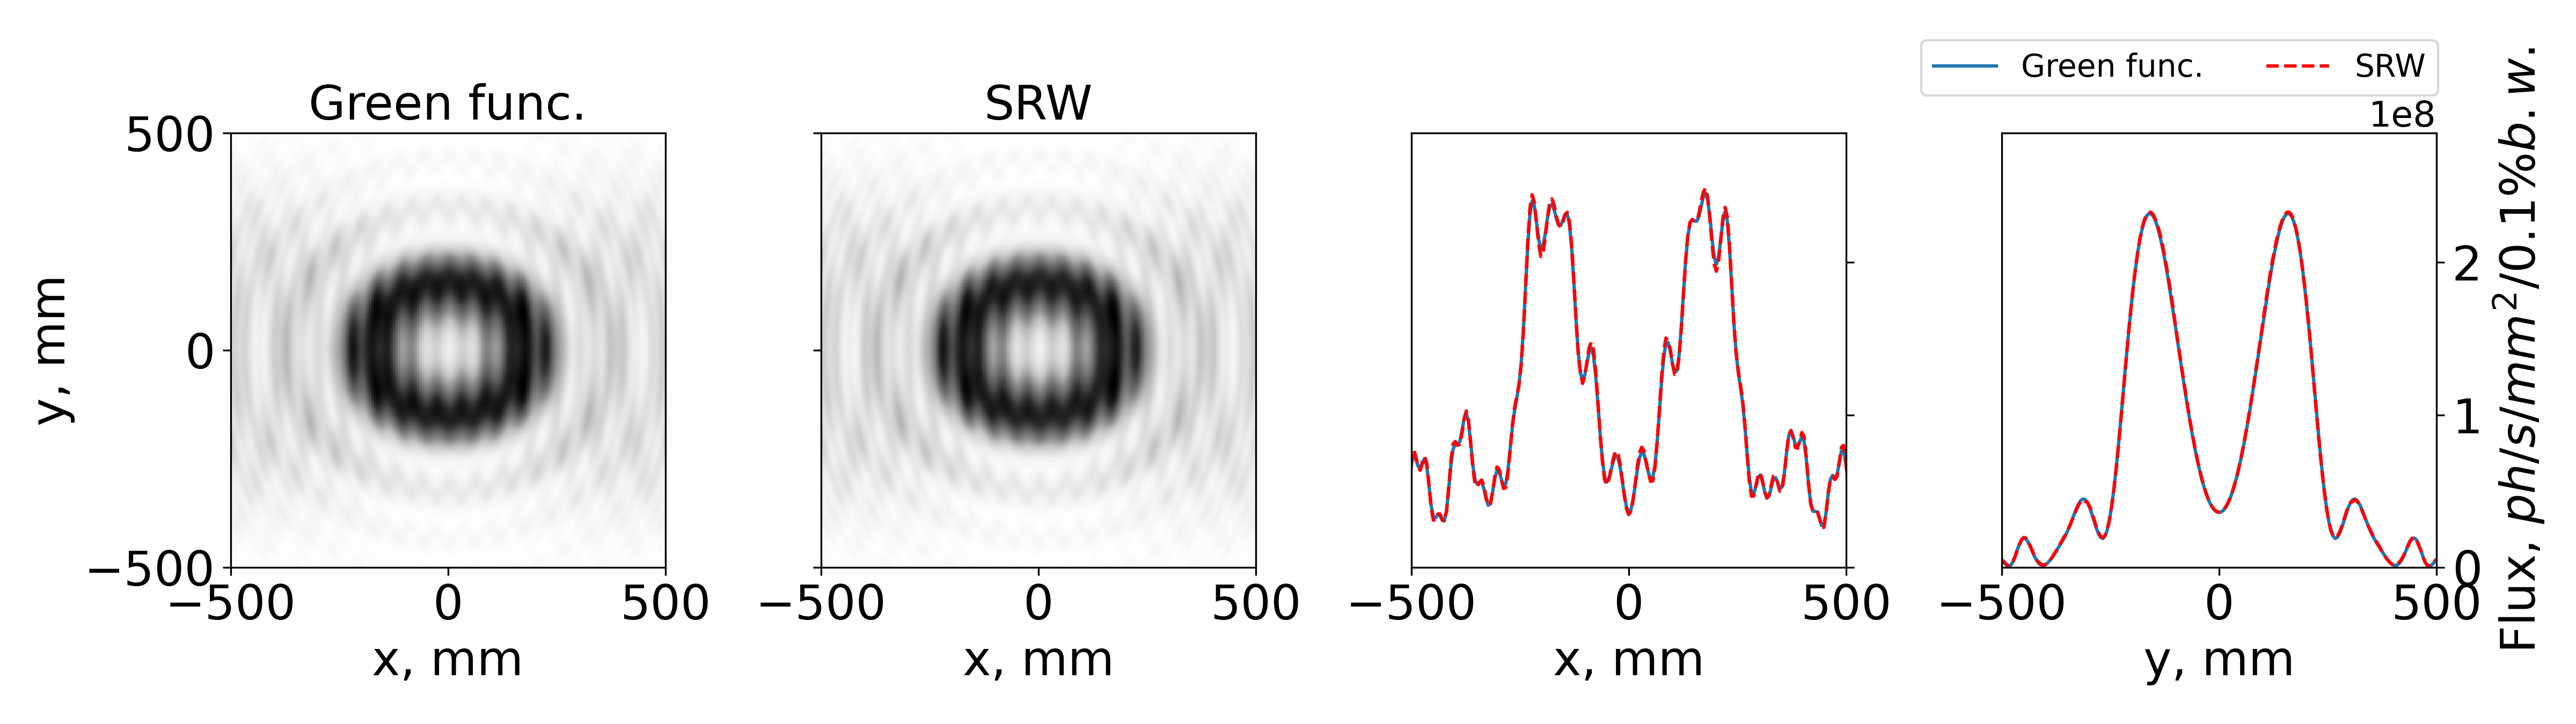
\includegraphics[width=0.95\linewidth]{content/images/5_THz_Source/bend.png}
        \captionsetup{justification=centering}
        \caption{Comparison of computational results from \rr{the developed code} and SRW for the radiation from the magnetic structure presented in Fig.~\ref{Fig:bending_magnet_figs} (arrangement of bending magnets). Total flux is presented for both polarization components.}
        \label{Fig:bend}
    \end{figure*}

    Firstly, it is observed that the integral exhibits a highly oscillatory behavior, as depicted in Fig.~\ref{Fig:bending_integral}. This characteristic can be discerned from the expression of the integral:
    \begin{align}
        \vec{\tilde{E}}_{\perp}(\vec{r}_{\perp 0}, z_0, \omega) = - \cfrac{i \omega e}{c^2}\int_{-\infty}^{\infty} dz' \frac{1}{z_0 - z'}
        \bigg[\bigg(\frac{v_x(z')}{c} - \cfrac{x_0 - x'(z')}{z_0 - z'}\bigg)\vec{e}_x + \bigg(\frac{v_y(z')}{c} - \cfrac{y_0 - y'(z')}{z_0 - z'}\bigg)\vec{e}_y\bigg] \times
        \cr \exp{\bigg[i\omega \bigg(\cfrac{(x_0 - x'(z'))^2 + (y_0 - y'(z'))^2}{2c(z_0 - z')} +  \cfrac{s(z')}{v} - \frac{z'}{c} \bigg)\bigg]}
        \label{Eq:free_space_Green_function_integral_simp}
    \end{align}
    As electrons diverge from the optical axis ($x, y = 0$ and $x_p, y_p = 0$), the phase increases, and the integral begins to oscillate. This behavior should be avoided in calculations, as the contributions from these parts are nearly zero, yet the high oscillations may lead to aliasing problems. In this specific simulation, the frequency of oscillation remains at a manageable level relative to the chosen mesh step size. 

    Secondly, one needs to be aware of the fact that, strictly speaking, it is not entirely correct to define only a part of the trajectory, e.g., from point $A$ to point $B$, as I have illustrated in Fig.~\ref{Fig:bending_traj}.(a). This actually represents a physical scenario where an electron appears at point $A$, accelerates from $0$ to $\beta$, flies to point $B$ across the given magnetic fields, then decelerates and disappears. This instant creation and disappearance of an electron correspond to the special case that I mentioned at the outset. Strictly speaking, one needs to integrate from $-\infty$ to $+\infty$ or within limits where the external segments: $[-\infty, A]$ and $[B, +\infty]$, contribute negligibly small value to the integral.In Fig.~\ref{Fig:bend}, the contributions from the edges are evident as the oscillations in the horizontal direction. One can observe that these edge sources point to the right and left, and one sees the interference of the bending magnets radiation with the edges. Again, this example is illustrative and highlights several issues that may occur when calculating synchrotron radiation. However, for the purpose of cross-checking of the developed code with well-established approaches, it is very valuable as it summarizes all the numerical and physics pitfalls. In the next subsection, I will present more trivial cases of three pole radiation and undulator radiation, and conclude the section with the illustrative case of entirely edge radiation case.
    
    \begin{figure}[h!]
    	\centering
        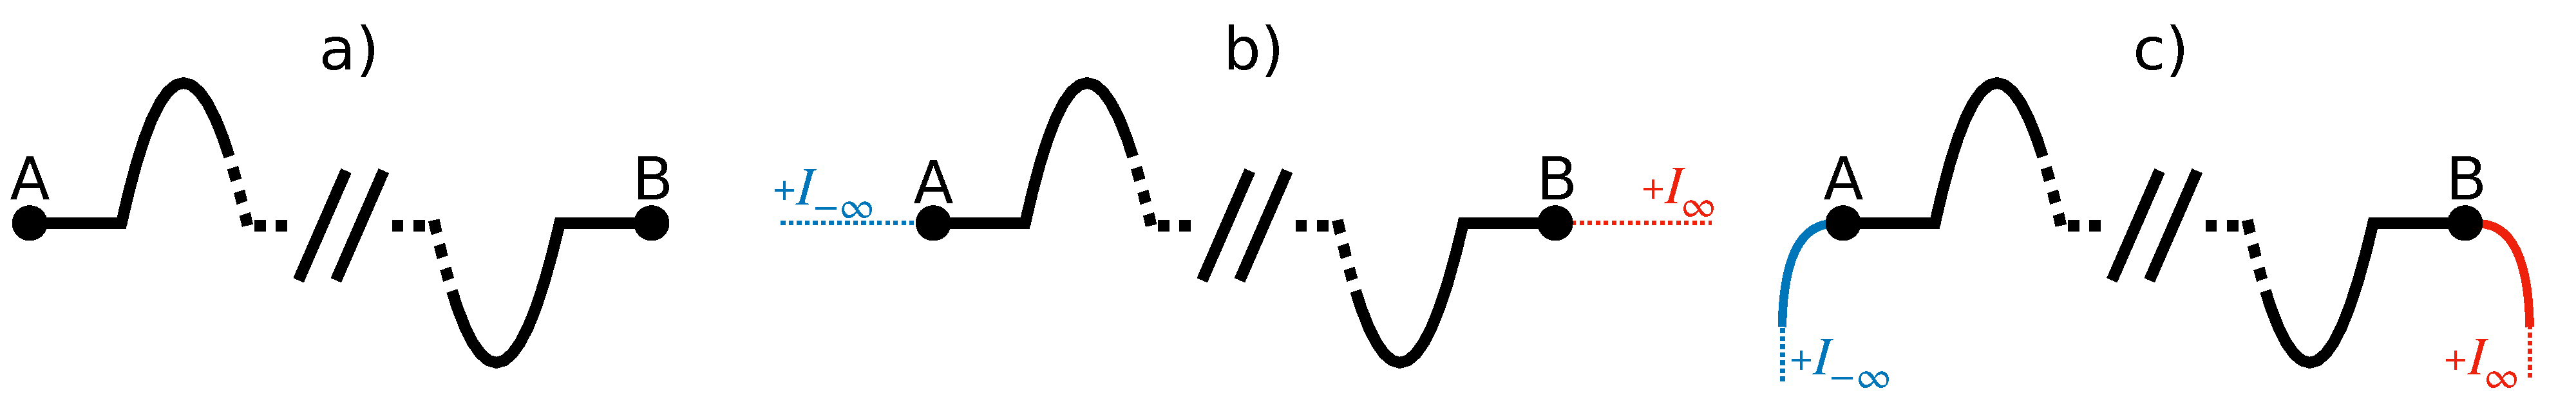
\includegraphics[width=0.95\linewidth]{content/images/5_THz_Source/integration_lim.pdf}
        \captionsetup{justification=centering}
        \caption{Schematic representation of the integration path over a magnetic structure. a) represents integration solely within the limits where the magnetic field is defined, i.e., from $A$ to $B$. b) shows the case when one semi-analytically estimates the contribution from the outer parts $[-\infty, A]$ and $[B, +\infty]$. c) represents a numerical trick on how to render this semi-analytical estimation negligible in codes where this estimation is performed automatically.}
        \label{Fig:integration_lim}
    \end{figure}
    
    One practical solution to this problem is to estimate these outer parts semi-analytically. The integral is split into three integration regions: $[-\infty, A]$, $[A, B]$, and $[B, +\infty]$, where $A$ and $B$ should be carefully chosen to avoid highly oscillatory behavior.
    \begin{align}
        \int_{-\infty}^{\infty} F e^{-i G} dz = \int_{-\infty}^{A} F e^{-i G} dz + \int_{A}^{B} F e^{-i G} dz + \int_{B}^{\infty} F e^{-i \omega G} dz
    \end{align}
    After performing a simple asymptotic integral expansion of the outer parts up to the second order, in accordance with a Filon-type method~\rr{cite}, one can obtain the follwing expression: \rr{correct formula}:
    \begin{align}
        \int_{-\infty}^{\infty} F e^{-i G} dz \approx \int_{A}^{B} F e^{-i G} dz + \bigg[ \cfrac{F}{i G'} + \cfrac{F'G' - FG''}{G'^3} e^{-i G}\bigg] \bigg |_{A}^{B}
        \label{Eq:integral_ev_semianalytical}
    \end{align}
    This semi-analytical estimation of the outer integral has not yet been incorporated into the developed code. This omission is partly due to the fact that, in the case of the general approach, one needs to first estimate the numerical derivatives, both first and second order, which can lead to a loss of accuracy and possible numerical artifacts, as well as demand careful implementation. For the sake of completeness in this presentation, I offer a comparison of the scenario where the contribution from the edges is not accounted for in \rr{the developed code}, against SRW, which can account for this contribution. This comparison is presented in Fig.~\ref{Fig:bend_edge_on}.
    \begin{figure*}[h!]
    	\centering
        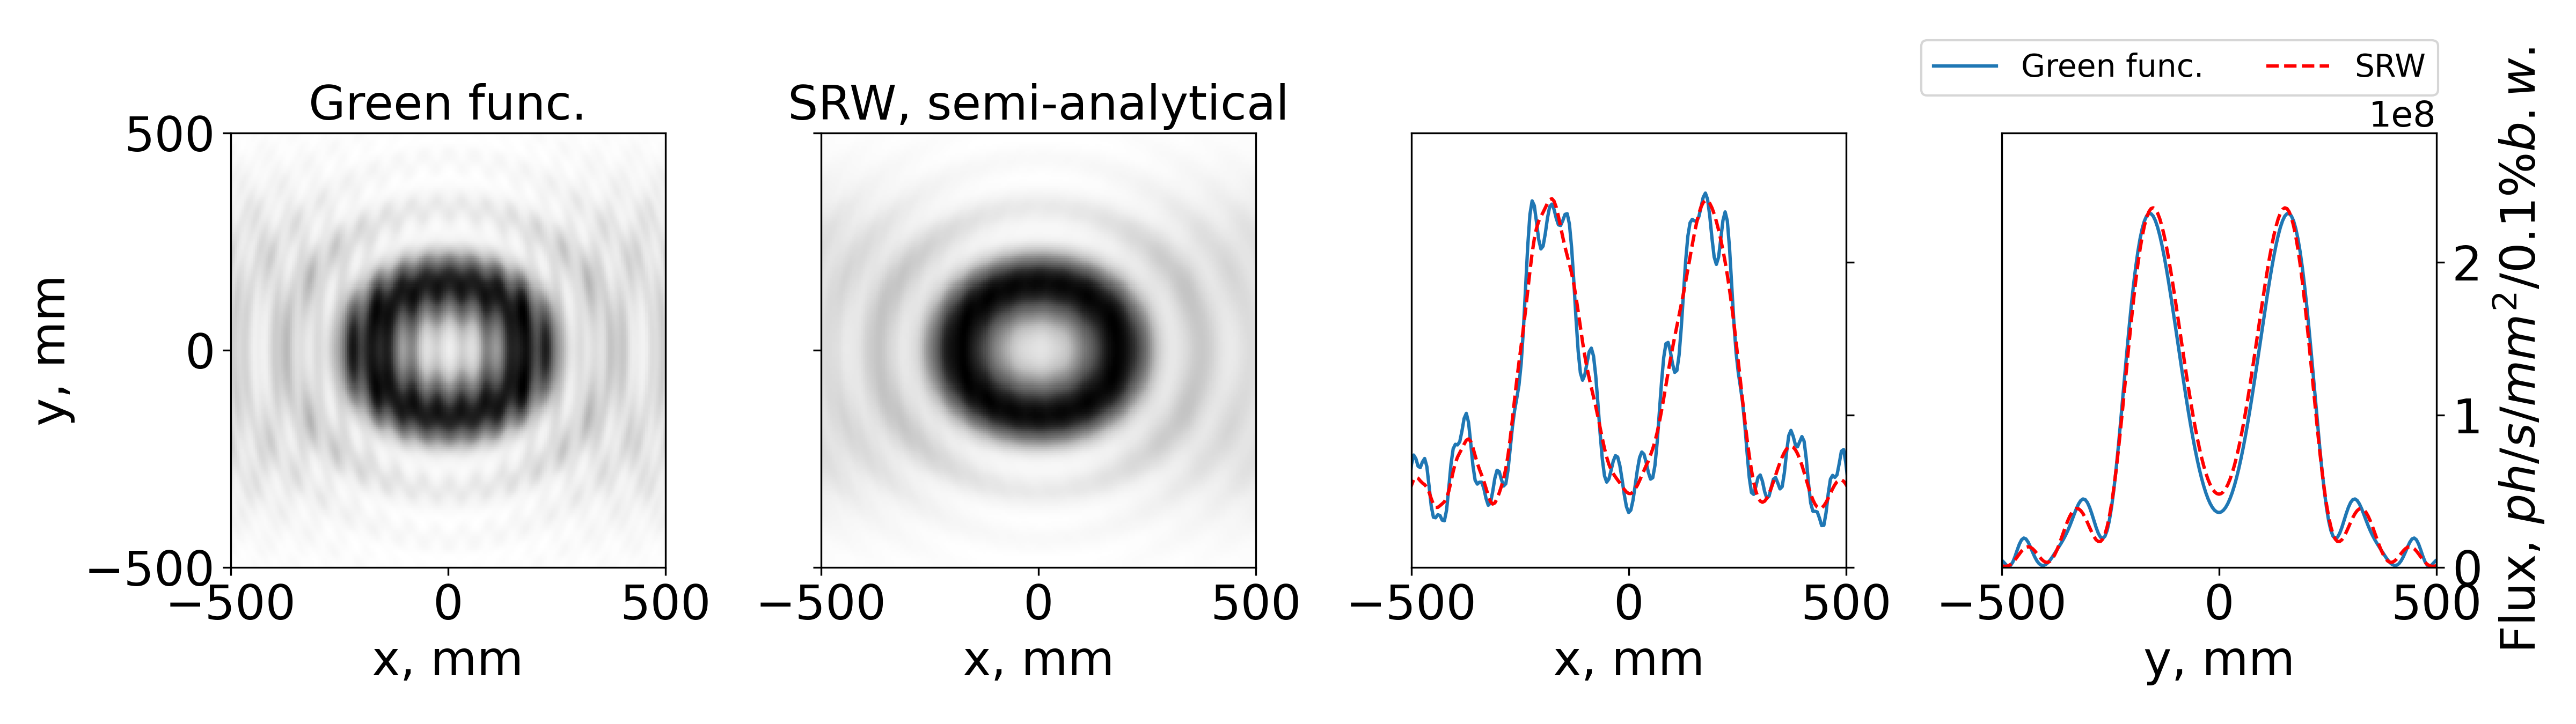
\includegraphics[width=0.95\linewidth]{content/images/5_THz_Source/bend_edge_on.png}
        \captionsetup{justification=centering}
        \caption{Comparison of computational results from \rr{the developed code} and SRW for the radiation from the magnetic structure presented in Fig.~\ref{Fig:bending_magnet} (arrangement of bending magnets). SRW accounts for the outer integral estimation, which is denoted in the corresponding figure as "SRW, semi-analytical". Total flux is presented for both polarization components.}
        \label{Fig:bend_edge_on}
    \end{figure*}
    
    Initially, I developed the code without being aware of this issue, and an evident incongruity in the results led to this in-depth cross-check. Thanks to a very productive discussion with E. Saldin and G. Geloni, who provided hints towards resolving this apparent paradox, and to the invaluable correspondence with O. Chubar, who explained the solution in more detail.
    
    In conducting cross-checks, it's crucial to recognize that other numerical codes might handle these terms differently. For instance, the formula is clearly implemented in the SRW code and, to the best of my knowledge, is tacitly applied in calculations within the SPECTRA and OCELOT toolkits. As mentioned, SRW allows for the semi-analytical estimation to be 'turned on' and 'off.' When set to 'off,' integration occurs only over the specified magnetic field from $A$ to $B$. In contrast, SPECTRA and OCELOT consistently account for this semi-analytical estimation, complicating cross-checks with \oo{the developed code}.~
    
    One way to overcome this issue is by adding instantaneous turns in the radiation trajectory at points $A$ and $B$ (e.g., via an abrupt magnetic field kick, as shown in Fig.~\ref{Fig:integration_lim}.(c)). This approach alters the estimation of the outer integrals, rendering their contribution negligible. Nonetheless, for a fair cross-check, it is sufficient to compare \rr{the developed} code with SRW only, since SPECTRA and OCELOT yield the same results as SRW when semi-analytical estimation is "on" and have been cross-checked against each other elsewhere \rr{cite}. Therefore, the cross-check will focus on the portion of the trajectory from $A$ to $B$, corresponding to the numerical case depicted in Fig.~\ref{Fig:integration_lim}.(a).
    
    Continuing the discussion, it is evident that there are two approaches to tackling the calculation of synchrotron radiation. The first approach involves defining a trajectory from $A$ to $B$, ensuring it is 'physical,' meaning the contribution from the edges is negligible. This method is the most straightforward but may lead to the emergence of highly oscillatory integrals, which require careful consideration. The second alternative involves semi-analytically evaluating the outer integral according to Eq.~\ref{Eq:integral_ev_semianalytical}. However, in this case, this estimation may not accurately represent the real magnetic configuration outside the defined range from $A$ to $B$, which can influence the resulting radiation distribution.

\subsubsection{Three pole radiation}
    In this subsection, I will present another numerical example featuring a three-pole device, as shown in Fig.~\ref{Fig:3pole_traj}. In this magnetic system, the first and the second magnetic field integrals are "closed", effectively returning the electron to $x, y = 0$ and $x_p, y_p = 0$. This makes the integrant to be zero, as illustrated in Fig.~\ref{Fig:3pole_traj}. Consequently, highly oscillatory behaviors are effectively suppressed, simplifying the integration process. However, this scenario is not entirely physical, as only part of the trajectory is defined. Thus, one can also observe the influence of the edge terms, evident in the characteristic interference circles depicted in Fig.~\ref{Fig:pole}. Nevertheless, this reinforces the cross-check as it represents a more challenging case to calculate
    \begin{figure*}[p]
        \centering
        \begin{subfigure}[c]{0.5\linewidth}  % [c] option for vertical centering
            \centering
            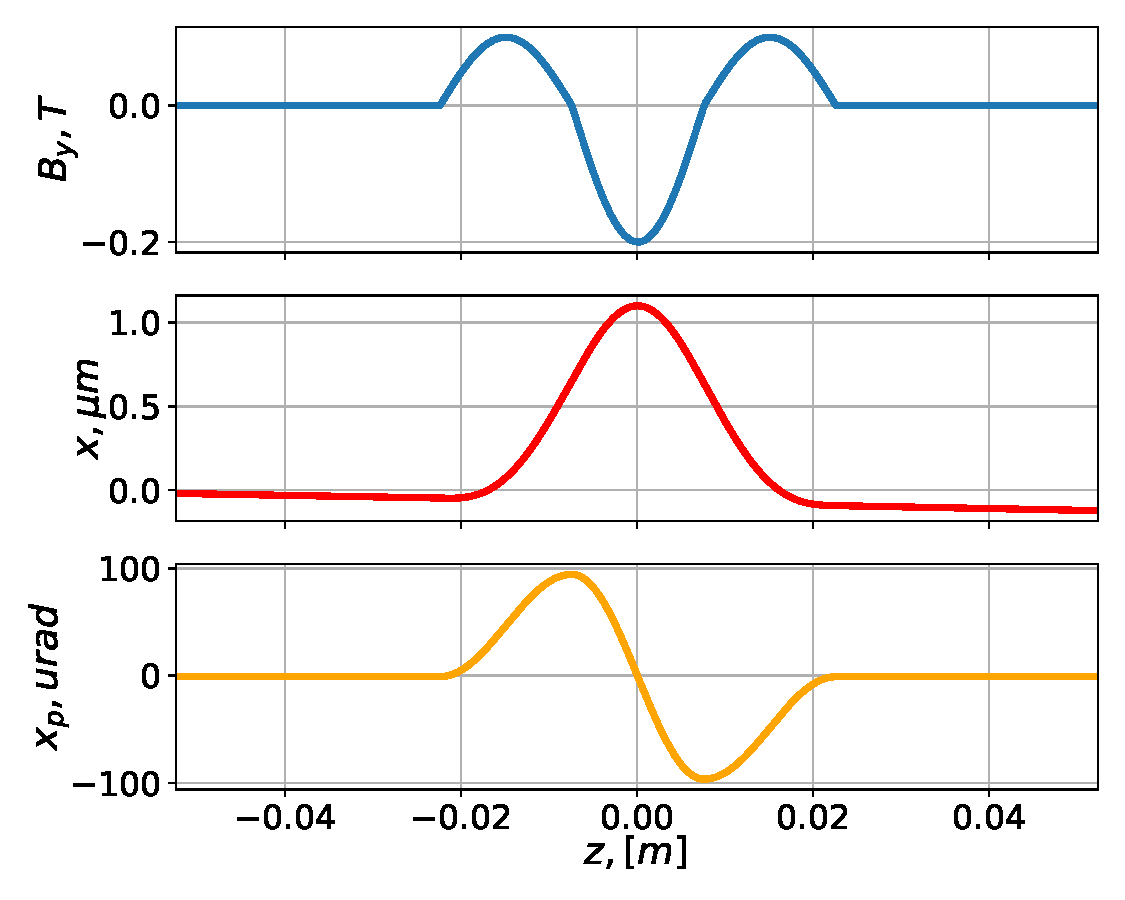
\includegraphics[width=\linewidth]{content/images/5_THz_Source/3pole_traj.pdf}
            \caption{From top to bottom: $y$ component of the magnetic field, $x$ component of the trajectory and $x_p$ is the angel of the electron's direction.} % Optional individual caption for the first subfigure
            \label{Fig:3pole_traj}
        \end{subfigure}%
        \begin{subfigure}[c]{0.5\linewidth}  % [c] option for vertical centering
            \centering
            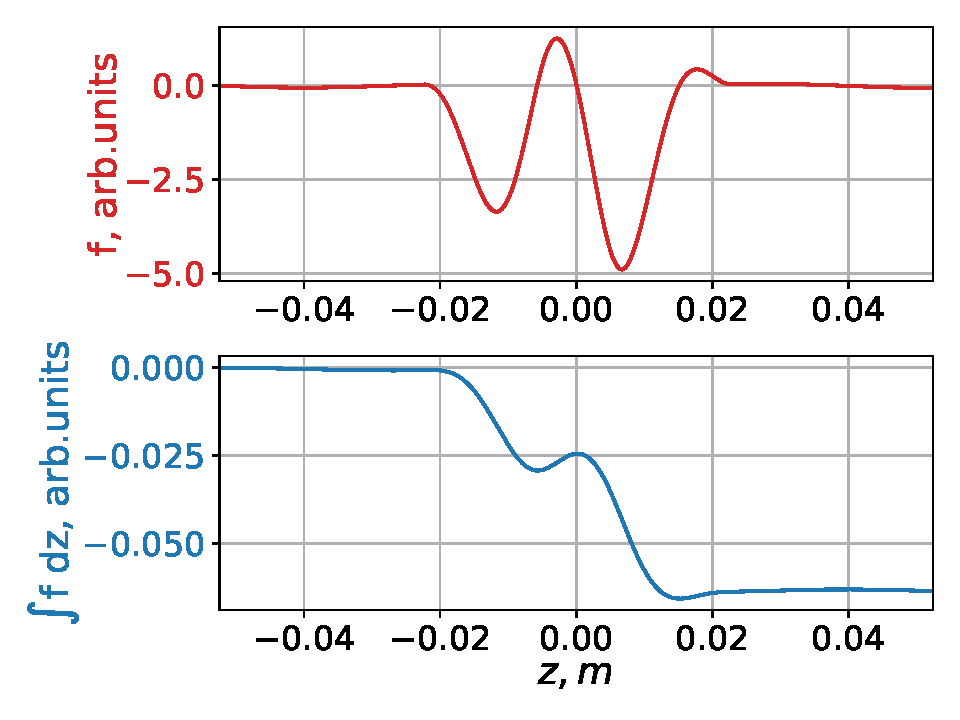
\includegraphics[width=\linewidth]{content/images/5_THz_Source/3pole_integral.pdf}
            \caption{Integrant value with respect to $z$ value and corresponding integral value for the three pole radiation.} % Optional individual caption for the second subfigure
            \label{Fig:3pole_integral}
        \end{subfigure}
        \caption{Three pole trajectory and integral evaluation with respect to the longitudinal coordinate.} % Optional overall caption            
        \label{Fig:3pole_figs}
    \end{figure*}
    
    \begin{figure*}[p]
    	\centering
        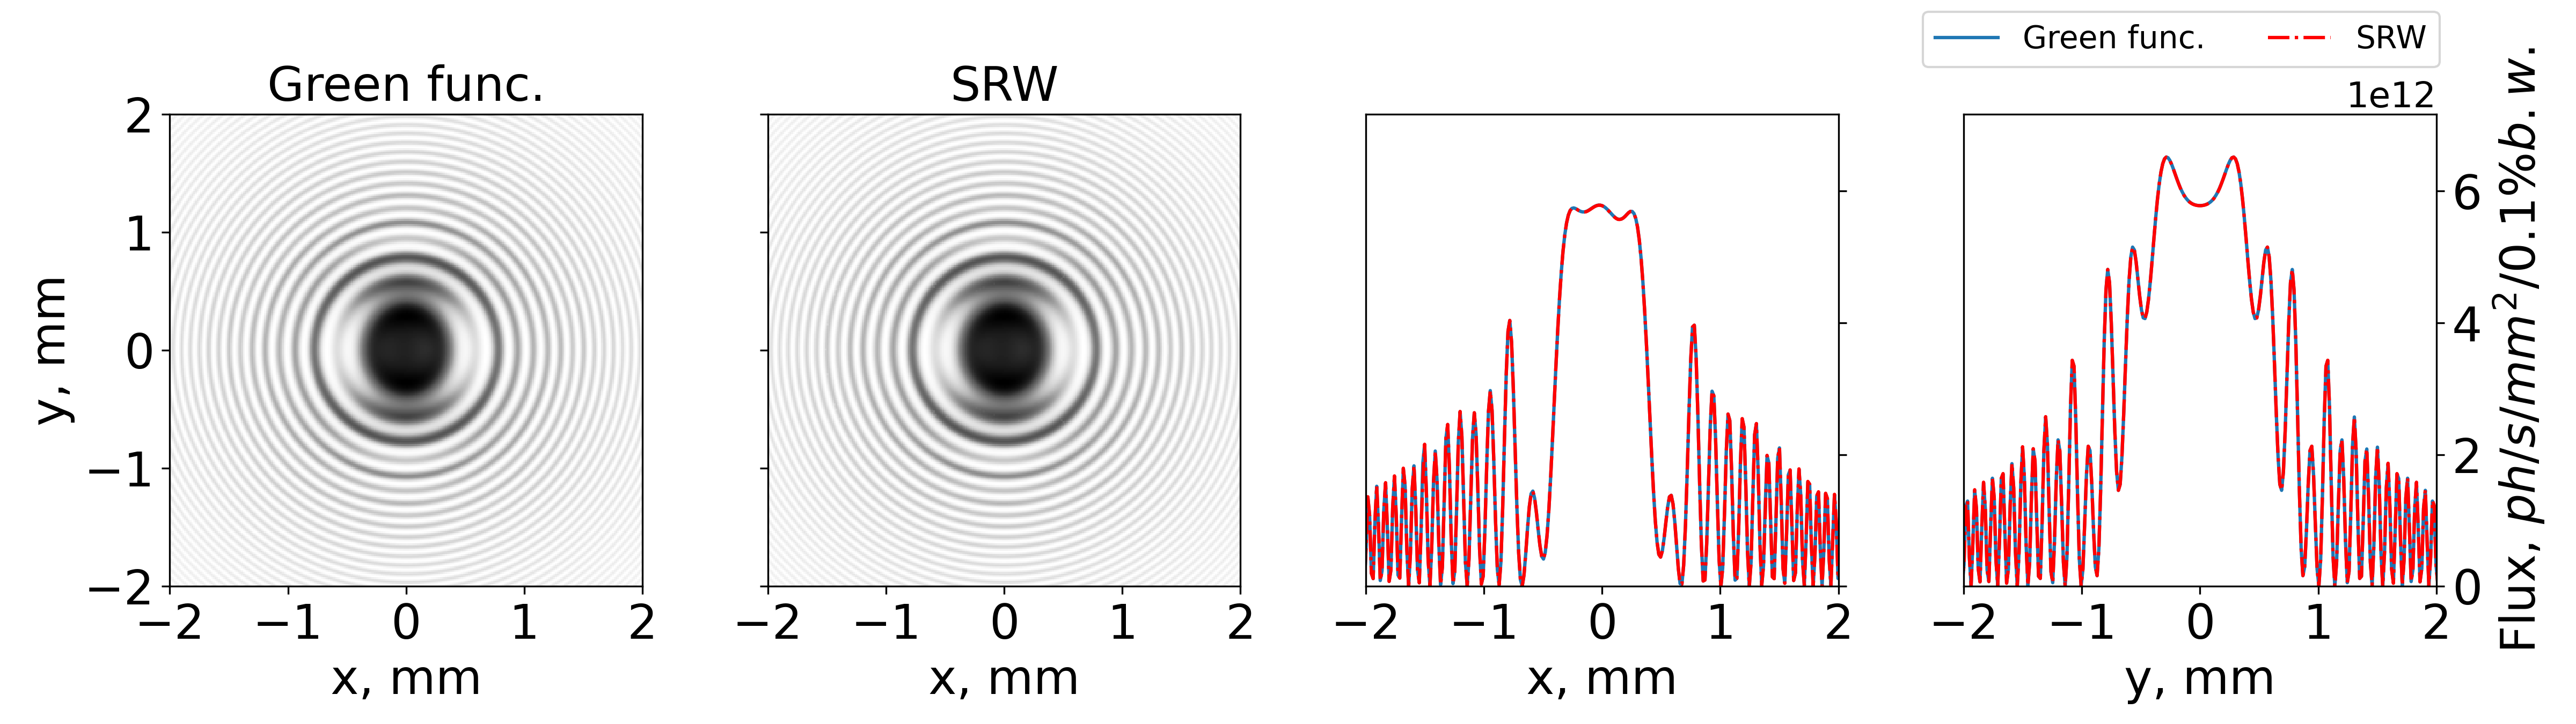
\includegraphics[width=0.95\linewidth]{content/images/5_THz_Source/3pole.png}
        \captionsetup{justification=centering}
        \caption{Comparison of computational results from \rr{the developed code} and SRW for the radiation from the magnetic structure presented in Fig.~\ref{Fig:pole} a three pole device.  Total flux is presented for both polarization components.}
        \label{Fig:pole}
    \end{figure*}

\subsubsection{Undulator radiation radiation}
    Another case that should be checked is undulator radiation, for example, from a magnetic field seen in Fig.~\ref{Fig:und_traj}. In undulators, the integral value adds up 'coherently' at each period (Fig.~\ref{Fig:und_integral}). This is essentially the unique property of undulator radiation that increases the power of radiation compared to a single pole, in proportion to the square of the number of undulator periods. In cases where the influence of the edge terms is barely noticeable on the total power distribution of the radiation in resonance (Fig.~\ref{Fig:und}), it is because the radiation from the device is an order of magnitude higher than that from the edges. However, it can be clearly seen for the $y$ polarization component, as depicted in Fig.~\ref{Fig:und_edge_on}. I need to note that to calculate the last case with SRW, it was necessary to add small straight sections before and after the undulator to proceed correctly with the semi-analytical estimation overwise it gives numerical artefacts.
    
    \begin{figure*}[p]
        \centering
        \begin{subfigure}[c]{0.5\linewidth}  % Use [c] for vertical centering
            \centering
            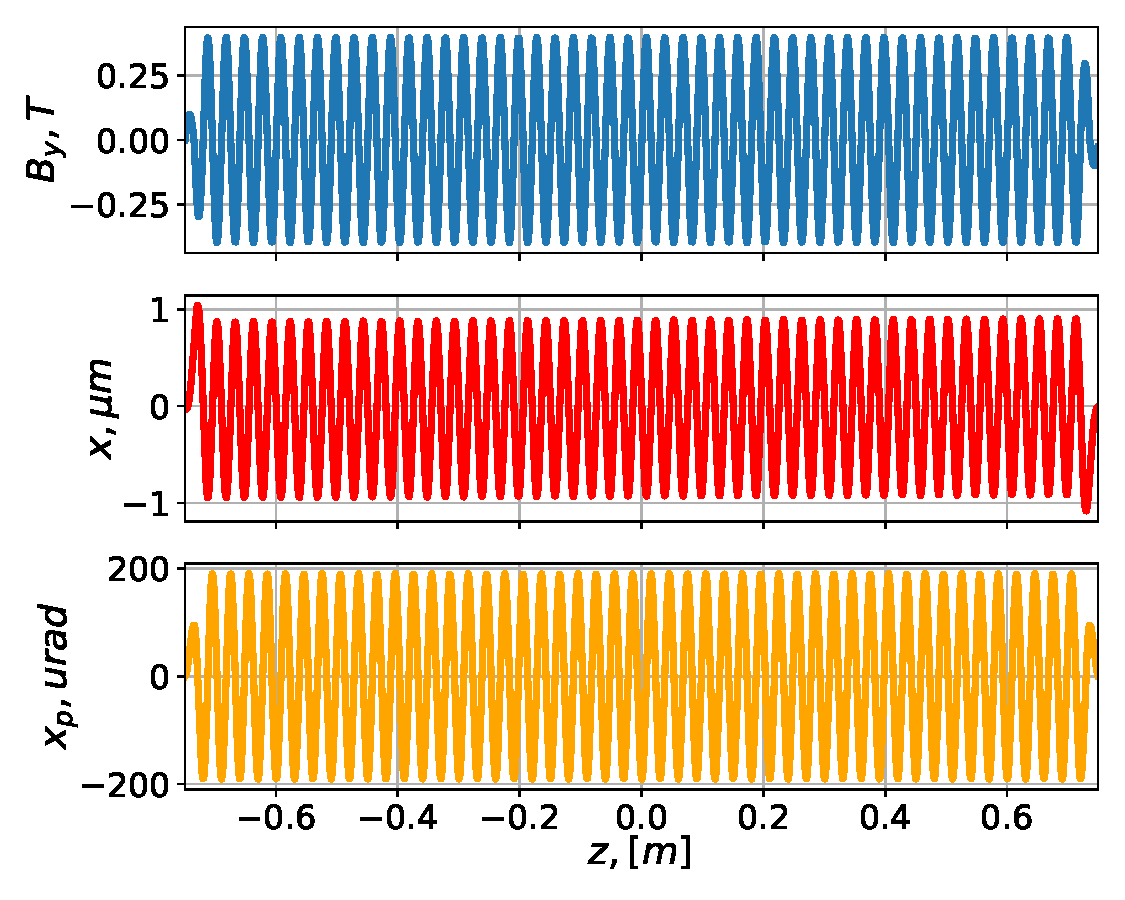
\includegraphics[width=\linewidth]{content/images/5_THz_Source/und_traj.pdf}
            \caption{From top to bottom: $y$ component of the magnetic field, $x$ component of the trajectory and $x_p$ is the angel of the electron's direction.} % Optional individual caption for the first subfigure
            \label{Fig:und_traj}
        \end{subfigure}%
        \begin{subfigure}[c]{0.5\linewidth}  % Use [c] for vertical centering
            \centering
            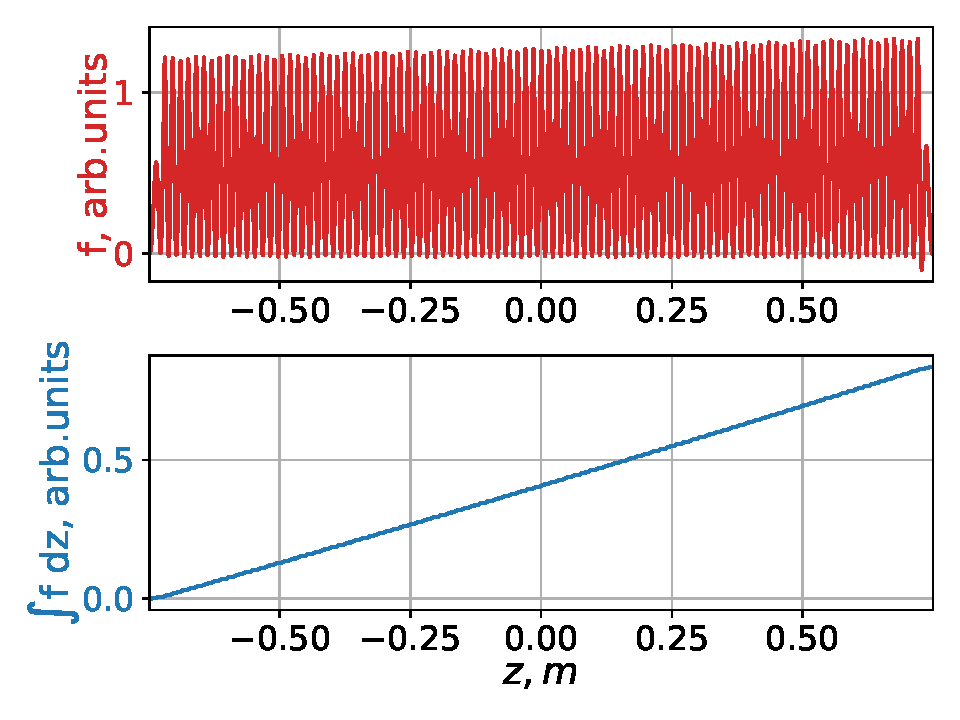
\includegraphics[width=\linewidth]{content/images/5_THz_Source/und_integral.pdf}
            \caption{Integrant value with respect to $z$ value and corresponding integral value for the undulator radiation.} % Optional individual caption for the second subfigure
            \label{Fig:und_integral}
        \end{subfigure}
            \caption{Undulator trajectory and integral evaluation with respect to the longitudinal coordinate.} % Optional overall caption            \label{fig:three_pole_figures}        \label{fig:und_figures}
        \label{Fig:und_integral_and_traj}
    \end{figure*}

    \begin{figure*}[p]
    	\centering
        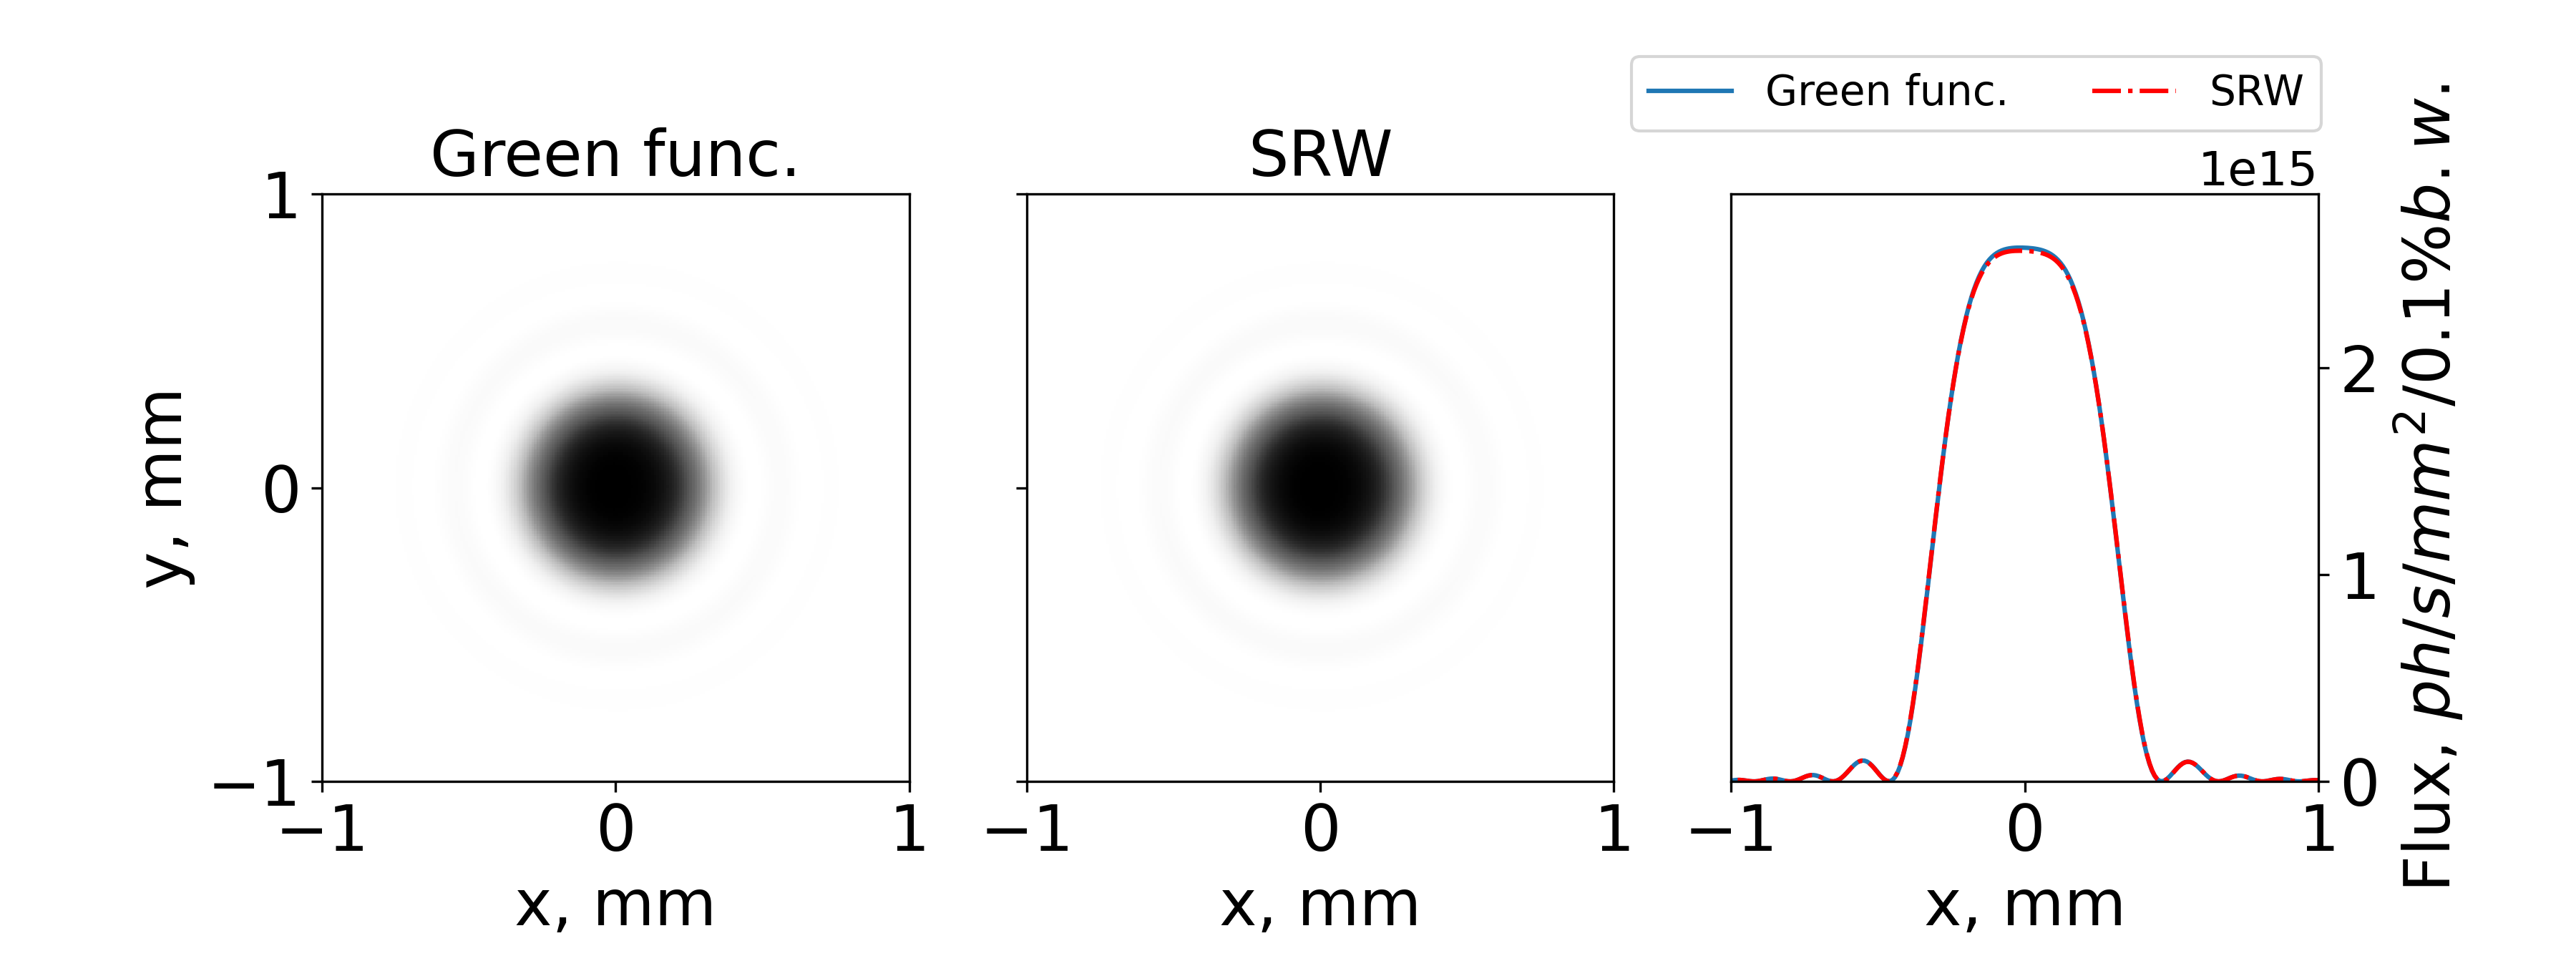
\includegraphics[width=0.71\linewidth]{content/images/5_THz_Source/und.png}
        \captionsetup{justification=centering}
        \caption{Comparison of computational result from different codes of radiation from the undulator radiation. Total flux is presented for both polarization components.}
        \label{Fig:und}
    \end{figure*}

    \begin{figure*}[p]
    	\centering
        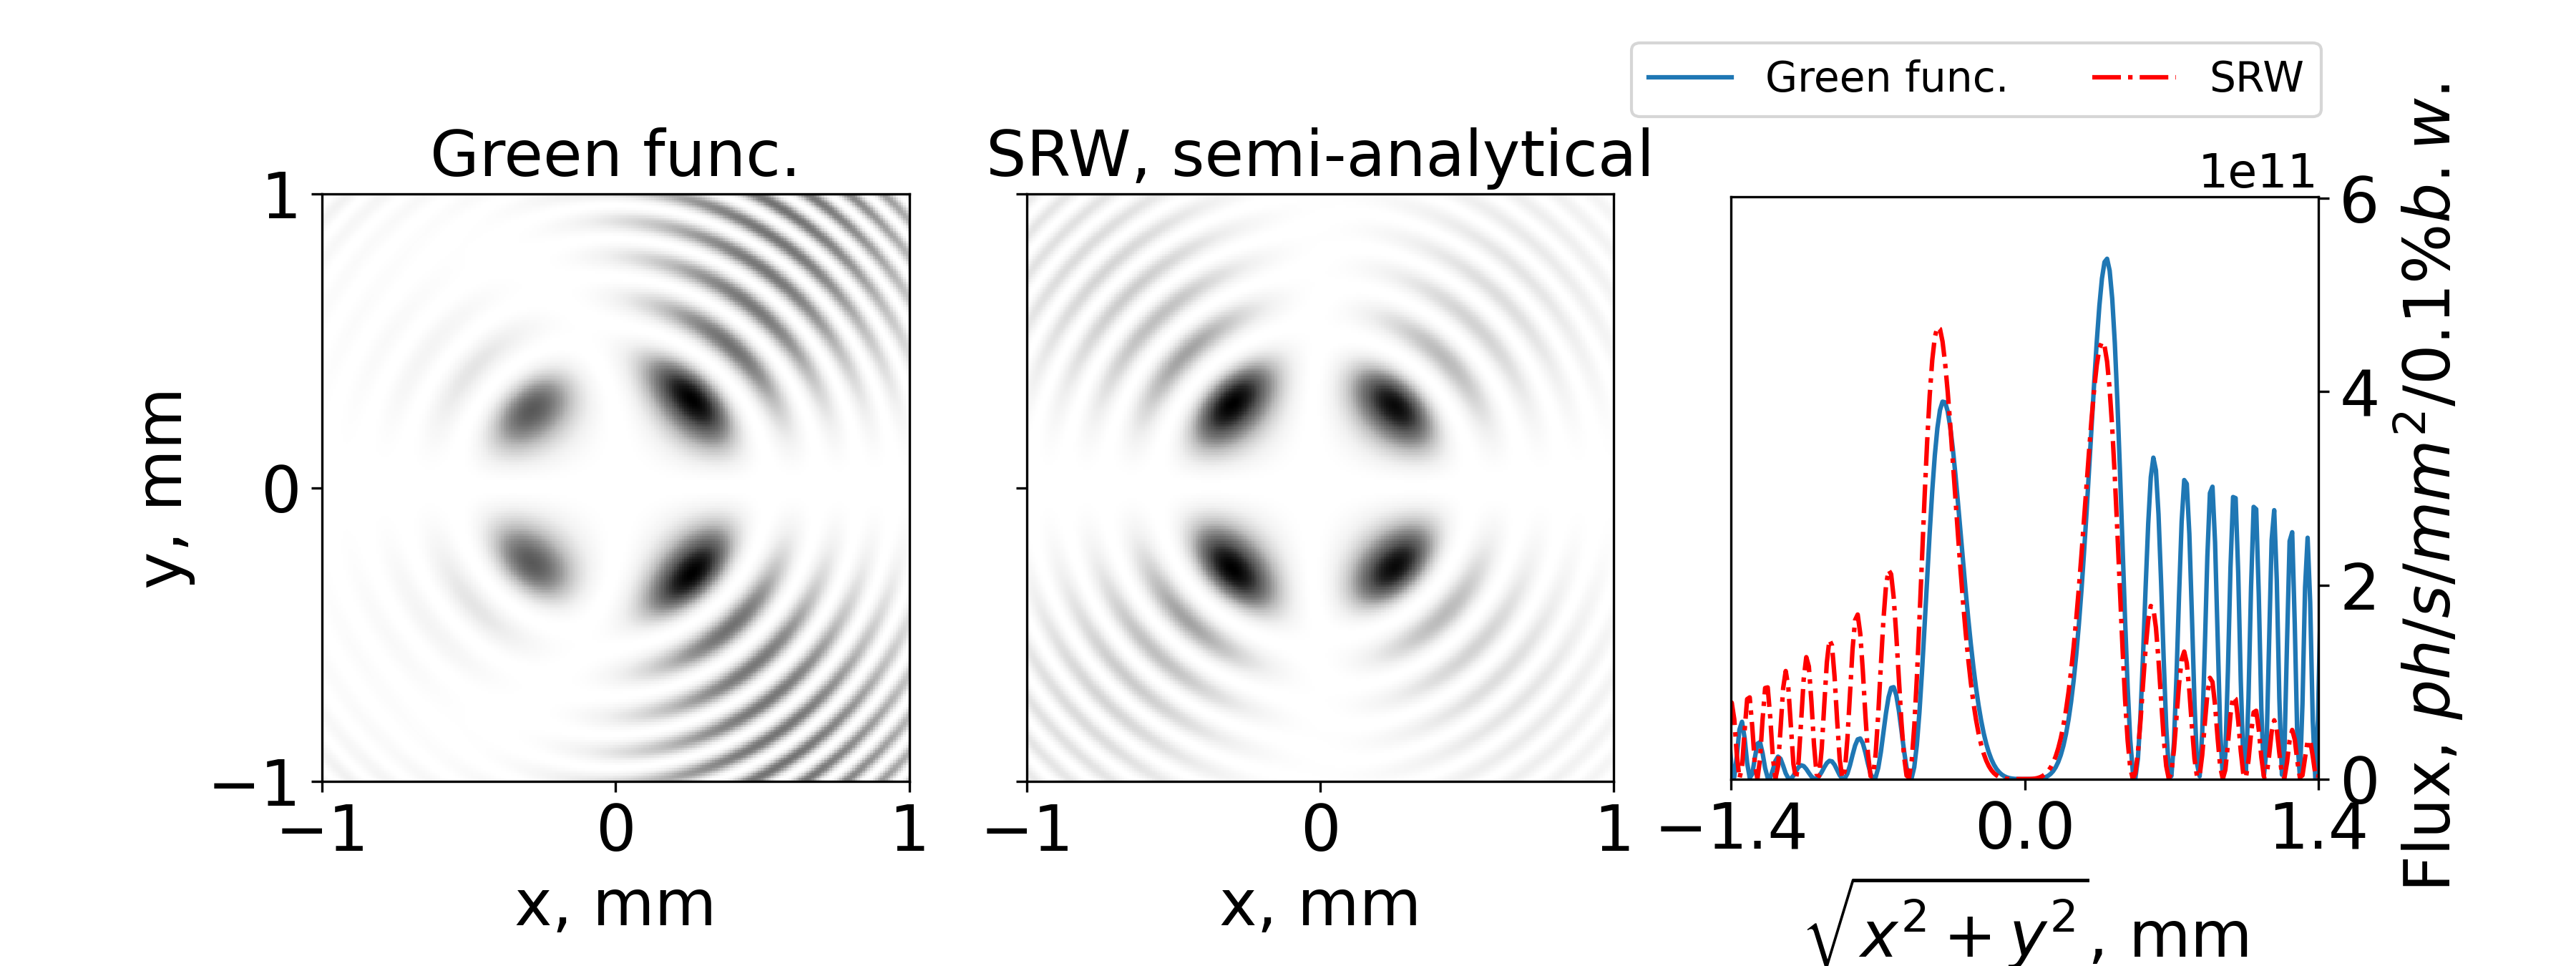
\includegraphics[width=0.71\linewidth]{content/images/5_THz_Source/und_edge_on.png}
        \captionsetup{justification=centering}
        \caption{Comparison of computational result from different codes of radiation from the undulator radiation. y-polarization flux is presented. The slice on the right subplot is presented for the diagonal cut.}
        \label{Fig:und_edge_on}
    \end{figure*}
    \pagebreak
    
\subsubsection{Straight section}
    I would like to conclude this section with the case of radiation from a straight section to demonstrate the contribution from the edges that I observed in the previous examples. By "straight section", I mean that the electron is created at point $A$, flies to $B$ in space with no magnetic field, and then disappears at $B$. This case represents radiation from two point sources situated at $A$ and $B$ and is described by the expression:   
    \begin{align}
        \vec{\widetilde{E}}_{AB}=\frac{ i \omega e L}{c^2 z}
        \exp\left[\frac{i \omega \theta^2 z}{2 c}\right] \vec{\theta} ~
        \mathrm{sinc}\left[\frac{\omega L}{4
        c}\left(\theta^2+\frac{1}{\gamma^2}\right)\right].
        \label{Eq:AB_analytical}    
    \end{align}
   Alternatively, this radiation can be understood using the integral expression where the sole contribution is from the 'gradient' term. I have depicted the cross-check of this case with SRW and the analytical expression in Eq.\ref{Eq:AB_analytical} in Fig.\ref{Fig:AB}.
    \begin{figure*}[h!]
    	\centering
        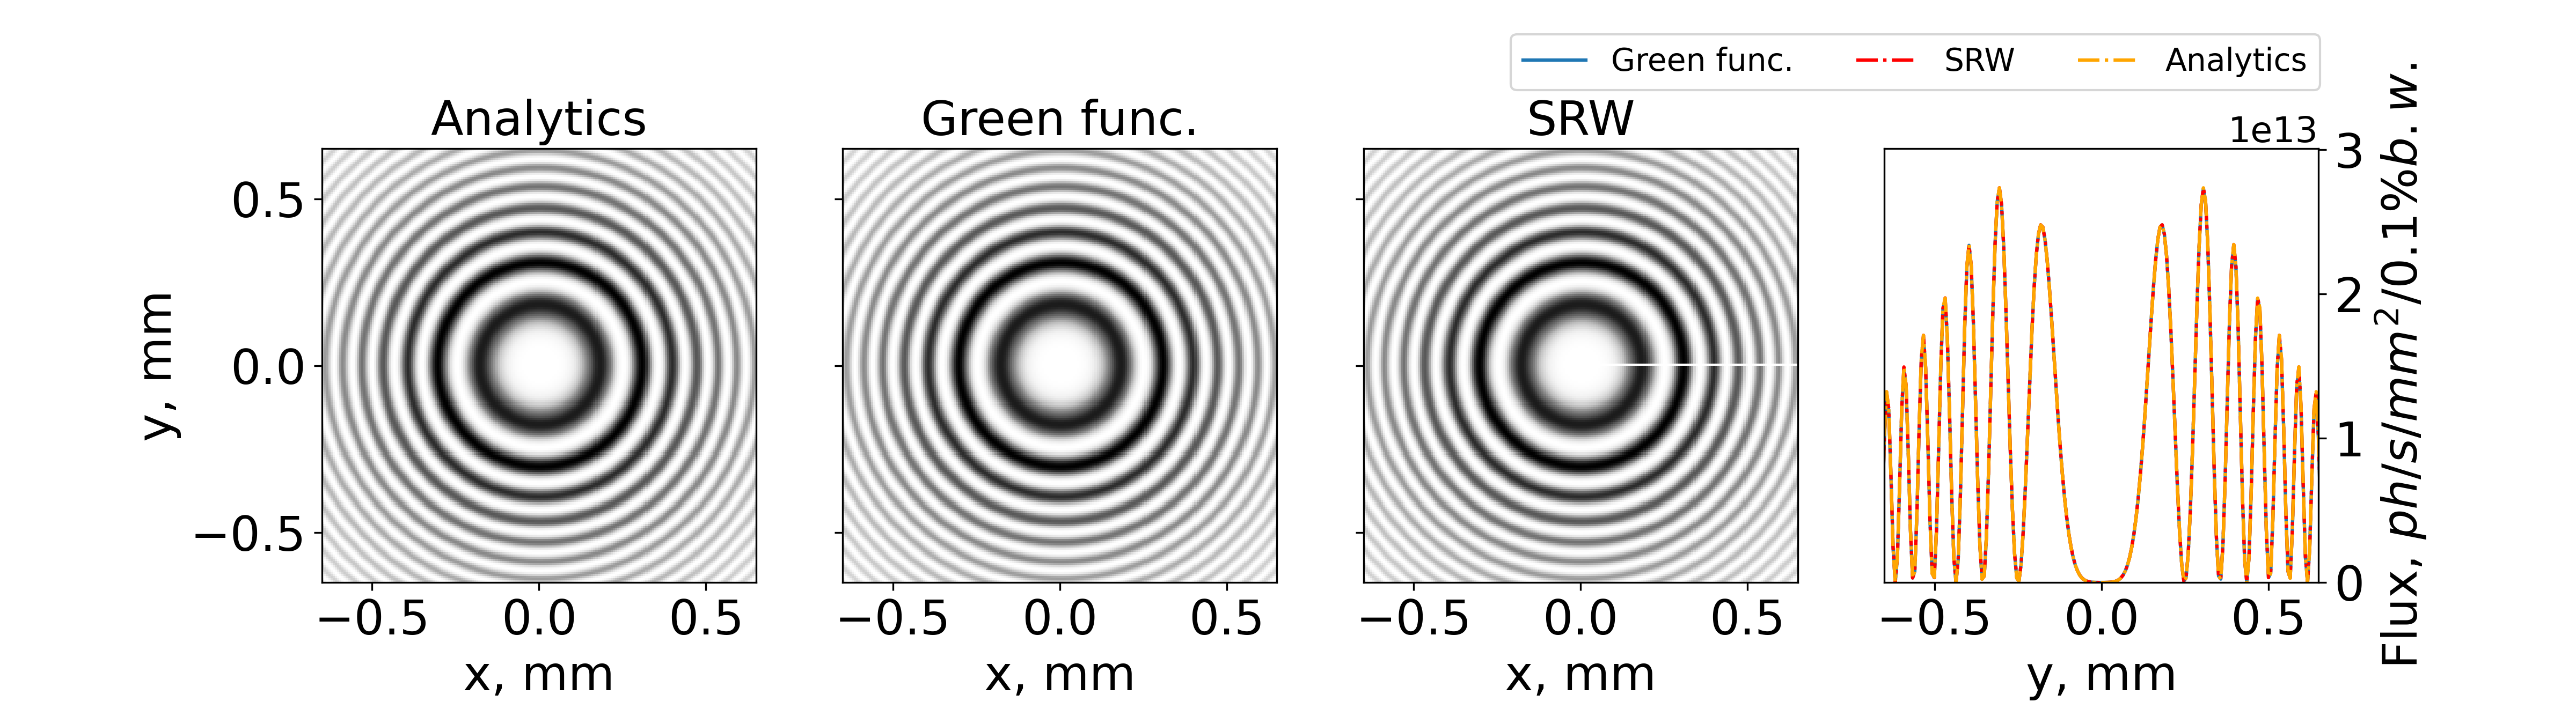
\includegraphics[width=0.99\linewidth]{content/images/5_THz_Source/AB.png}
        \captionsetup{justification=centering}
        \caption{Comparison of computational result from different codes of radiation from a straight section.}
        \label{Fig:AB}
    \end{figure*}
    
    These cases I have presented in this section demonstrate the applicability of the chosen approach of an integrator that can accept a Green function as input and perform integration (as well as taking derivatives from the Green's function). For this case of the free space Green's function, it has shown certain robustness in calculating the 'gradient' term. The next step in these cross-checks is to calculate examples using the circular waveguide Green's function.
    
\subsection{Circular waveguide Green's function}
    In this section I will present the result of the calculations using the circular waveguide Green's function and the cross-check of this results with asymptotic and analytical expressions. 

    The author of \rr{cite} represent the Green's function for the circular waveguide in the following form:
    \begin{eqnarray}
        &&G\left(\vec{r}_\bot,\vec{r'}_\bot,z-z'\right) = \frac{c}{2 i
        \omega} \sum_{m=0}^{\infty}\sum_{k=1}^{\infty}
        \left(A^{TE}_{mk}\right)^2 \left(\frac{\mu_{mk}}{2 R }\right)^2
        \exp\left[-\frac{i c (z-z')}{2\omega R^2 } \mu_{mk}^2\right] \cr
        && \times \left\{\left[\begin{array}{c} J_{m-1}(\mu_{mk}r/R)
        \cos[(m-1)\phi]+J_{m+1}(\mu_{mk}r/R) \cos[(m+1)\phi]
        \\
        -J_{m-1}(\mu_{mk}r/R) \sin[(m-1)\phi]+J_{m+1}(\mu_{mk}r/R)
        \sin[(m+1)\phi]
        \end{array}\right] \right. \cr && \left. \otimes \left[\begin{array}{c} J_{m-1}(\mu_{mk}r'/R)
        \cos[(m-1)\phi']+J_{m+1}(\mu_{mk}r'/R) \cos[(m+1)\phi']
        \\
        -J_{m-1}(\mu_{mk}r'/R) \sin[(m-1)\phi']+J_{m+1}(\mu_{mk}r'/R)
        \sin[(m+1)\phi']
        \end{array}\right] \right. \cr && \left. +
        \left[\begin{array}{c} -J_{m-1}(\mu_{mk}r/R)
        \sin[(m-1)\phi]-J_{m+1}(\mu_{mk}r/R) \sin[(m+1)\phi]
        \\
        -J_{m-1}(\mu_{mk}r/R) \cos[(m-1)\phi]+J_{m+1}(\mu_{mk}r/R)
        \cos[(m+1)\phi]
        \end{array}\right] \right. \cr && \left. \otimes
        \left[\begin{array}{c} -J_{m-1}(\mu_{mk}r'/R)
        \sin[(m-1)\phi']-J_{m+1}(\mu_{mk}r'/R) \sin[(m+1)\phi']
        \\
        -J_{m-1}(\mu_{mk}r'/R) \cos[(m-1)\phi']+J_{m+1}(\mu_{mk}r'/R)
        \cos[(m+1)\phi']
        \end{array}\right]\right\}
        \cr && + \frac{c}{2 i \omega}
        \sum_{m=0}^{\infty}\sum_{k=1}^{\infty} \left(A^{TM}_{mk}\right)^2
        \left(\frac{\nu_{mk}}{2 R }\right)^2 \exp\left[-\frac{i c
        (z-z')}{2\omega R^2 } \nu_{mk}^2\right] \cr && \times
        \left\{\left[\begin{array}{c} J_{m-1}(\nu_{mk}r/R)
        \sin[(m-1)\phi]-J_{m+1}(\nu_{mk}r/R) \sin[(m+1)\phi]
        \\
        J_{m-1}(\nu_{mk}r/R) \cos[(m-1)\phi]+J_{m+1}(\nu_{mk}r/R)
        \cos[(m+1)\phi]
        \end{array}\right] \right. \cr && \left. \otimes \left[\begin{array}{c} J_{m-1}(\nu_{mk}r'/R)
        \sin[(m-1)\phi']-J_{m+1}(\nu_{mk}r'/R) \sin[(m+1)\phi']
        \\
        J_{m-1}(\nu_{mk}r'/R) \cos[(m-1)\phi']+J_{m+1}(\nu_{mk}r'/R)
        \cos[(m+1)\phi']
        \end{array}\right] \right. \cr && \left. +
        \left[\begin{array}{c} J_{m-1}(\nu_{mk}r/R)
        \cos[(m-1)\phi]-J_{m+1}(\nu_{mk}r/R) \cos[(m+1)\phi]
        \\
        -J_{m-1}(\nu_{mk}r/R) \sin[(m-1)\phi]-J_{m+1}(\nu_{mk}r/R)
        \sin[(m+1)\phi]
        \end{array}\right] \right. \cr && \left. \otimes
        \left[\begin{array}{c} J_{m-1}(\nu_{mk}r'/R)
        \cos[(m-1)\phi']-J_{m+1}(\nu_{mk}r'/R) \cos[(m+1)\phi']
        \\
        -J_{m-1}(\nu_{mk}r'/R) \sin[(m-1)\phi']-J_{m+1}(\nu_{mk}r'/R)
        \sin[(m+1)\phi']
        \end{array}\right]\right\}~.
        \label{Eq:Circular_waveguide_green_function}
    \end{eqnarray}
    This expression should be substituted in Eq.~\ref{Eq:field_integral_tensor_full}. The first one and quite natural numerical cross-check is to let the radius of the waveguide be large and compare the result with the case of the free space Green function. 

\subsubsection{Free space limit}
    The next cross-check involves comparing the calculation results when the radius of the waveguide is large ($R = 1$~m). A radius of $1$~m, rather than a larger size, was chosen based on the reasoning that a larger radius would result in different transverse mode content and an increased number of $k$ modes that require summation. The selected radius of $1$~m is deemed sufficient for a demonstrative cross-check. One would expect that the radiation with the waveguide Green's function should result in the same spectral distribution as the free space Green function in the limit of large radius. For this calculation, I chose to use a three-pole device (a phase shifter), with the length of a pole being $0.45$~m and the magnetic field of the central pole at $2$~T and the side poles at $1$~T. I calculated spectral flux distribution and the result of the cross-check is presented in Fig.~\ref{Fig:free_space_limit}. 
    \begin{figure*}[h]
    	\centering
        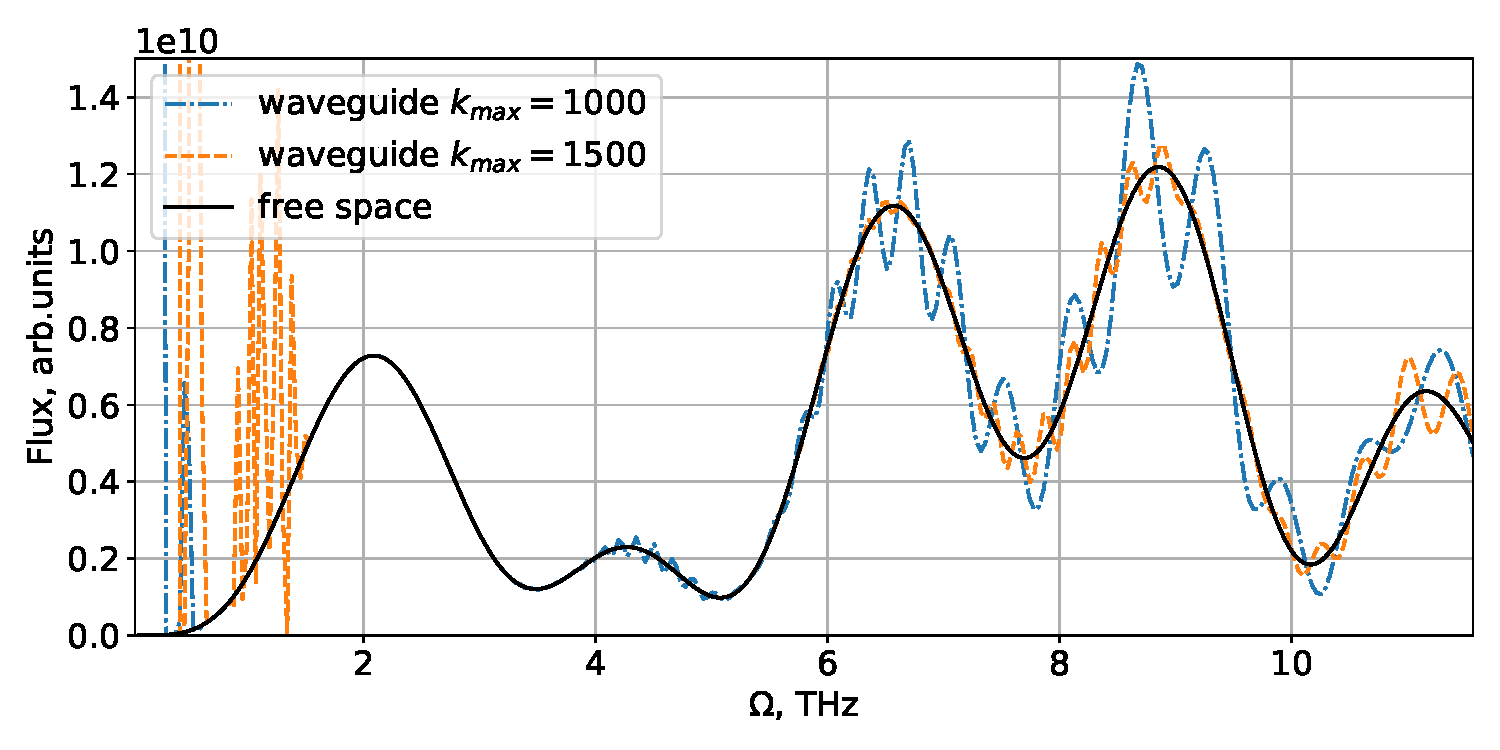
\includegraphics[width=0.8\linewidth]{content/images/5_THz_Source/free_space_limit.pdf}
        \captionsetup{justification=centering}
        \caption{The on-axis spectral flux from a three-pole device was calculated using the free space Green's function (represented by the black solid line) and the circular waveguide Green's function, taking into account different amounts of transverse modes: a blue dash-dotted line for 1000 modes and a dashed line for 1500 modes.}
        \label{Fig:free_space_limit}
    \end{figure*}
    
    The presented distribution can be divided into three parts. At the low end of radiation frequencies, there is a mismatch that can be explained by the appearance of highly oscillatory integrals. As one calculates higher mode number contributions, one can see that the exponent's argument starts to grow as well, along with $\mu_{mk}$ and $\nu_{mk}$. Then, there is a region where the two lines coincide — the behavior one would expect. Additionally, one observes an oscillatory behavior that indicates more modes should be summed, as can be seen when comparing the blue dashed-dotted line with the orange dashed line.

    It is relatively easy to cross-check on-axis spectral flux distributions because all transverse modes with a number higher than $m=1$ are equal to zero, as evidenced by the expression for the Green's function. This significantly simplifies the cross-check process, but it is still necessary to verify as general a case as possible. In the next section, I will present a cross-check of a real-sized waveguide against the analytical derivation that was made in~\rr{cite}.
    
\subsubsection{Spatial distribution}
    For this cross-check I chose an undulator with ten periods, the period length is $0.9$~m and the max magnetic field value is $2$~T. The magnetic field distribution does not have any end correction coils. This is made for the fair comparison as the analytical distribution is calculated for an idealized sin-like field distribution. I present this comparison in Fig.~\ref{Fig:pipe_check_2D} and the cross-section in Fig.~\ref{Fig:pipe_check_1D}.
    \begin{figure*}[p]
    	\centering
        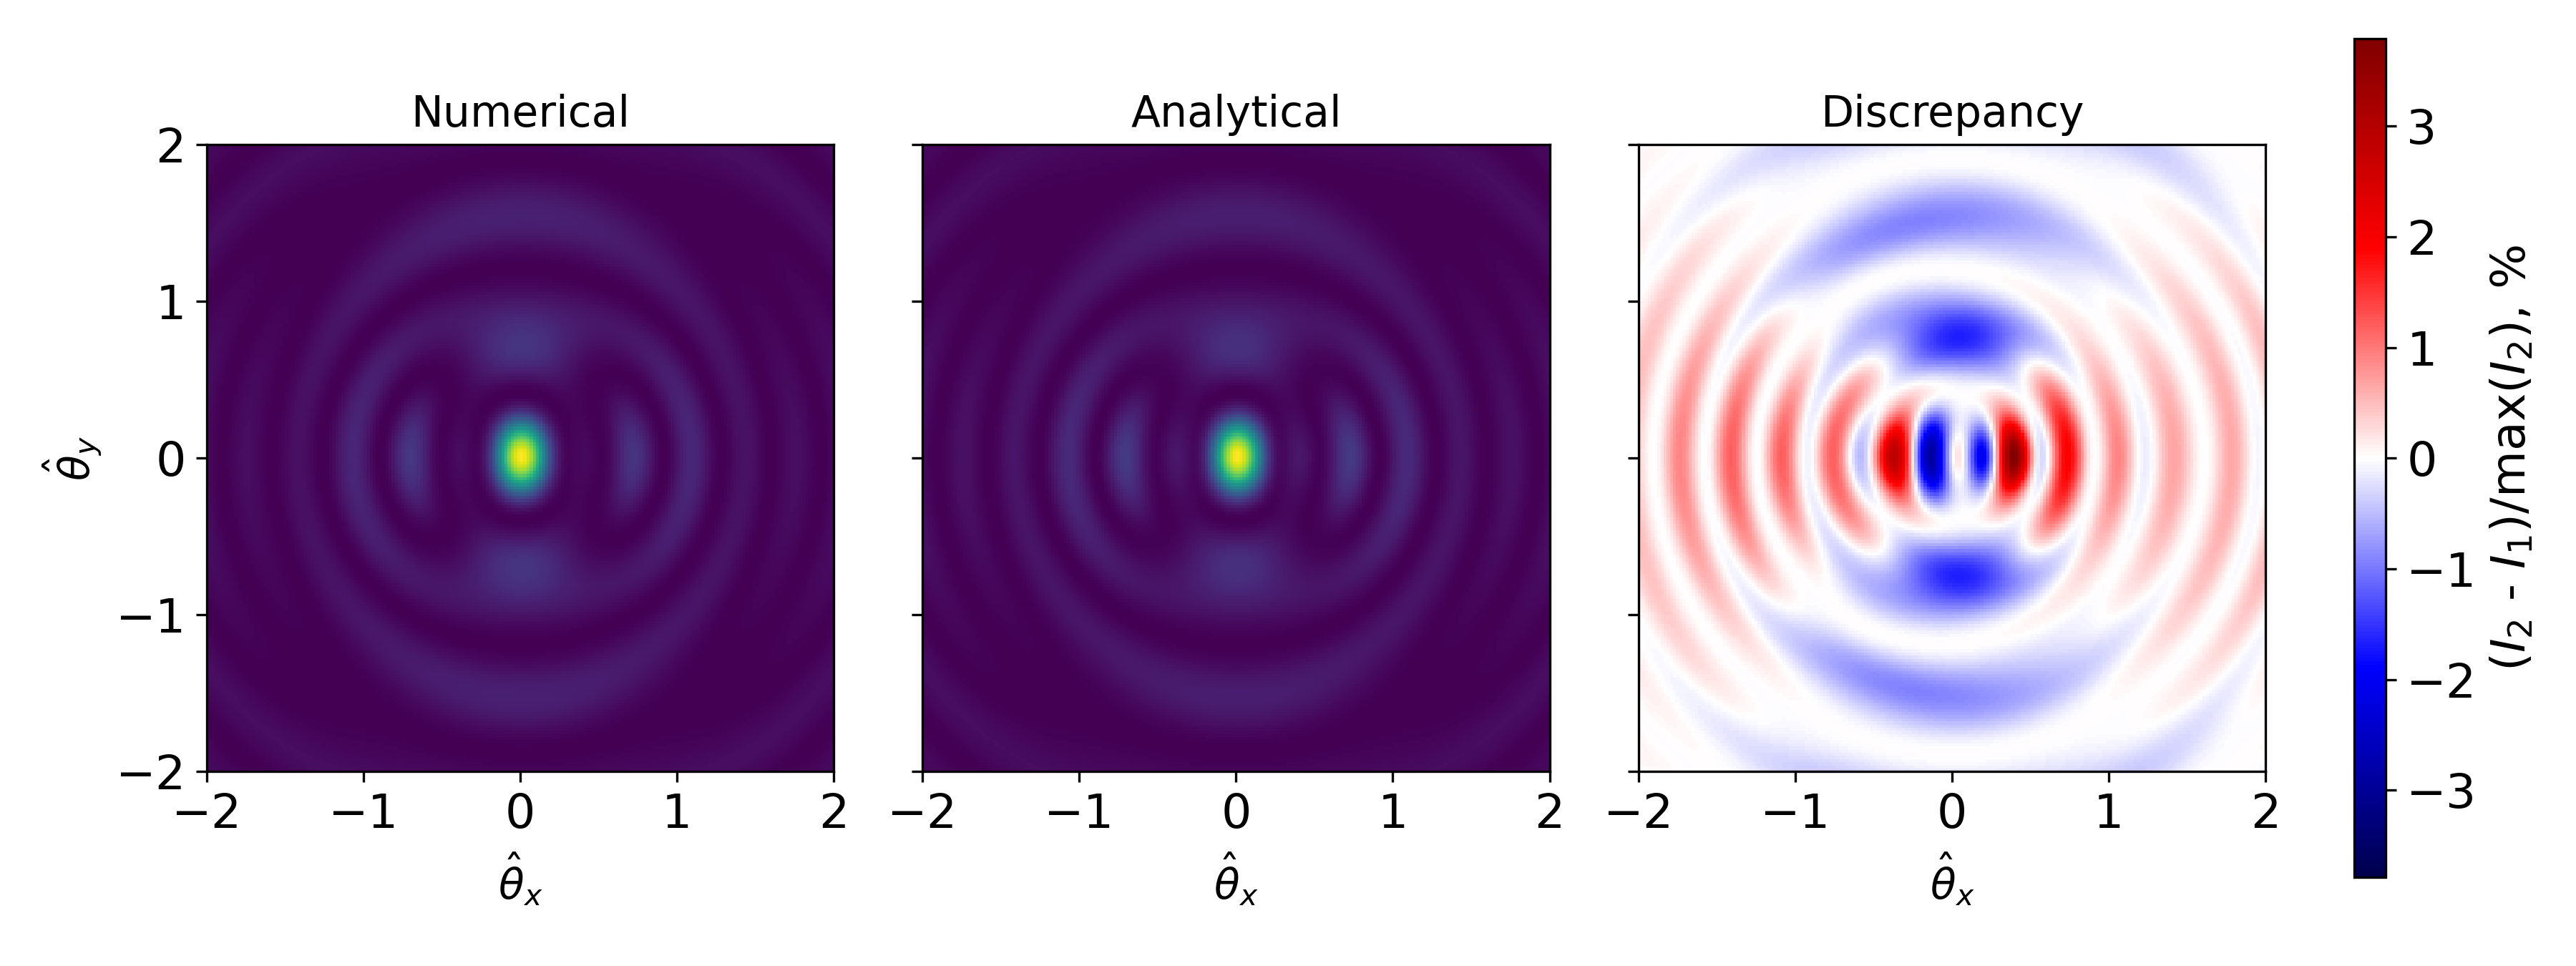
\includegraphics[width=0.99\linewidth]{content/images/5_THz_Source/pipe_check_2D.png}
        \captionsetup{justification=centering}
        \caption{Spatial distribution of radiation in the far zone from a ten period undulator in a waveguide.}
        \label{Fig:pipe_check_2D}
    \end{figure*}
    \begin{figure*}[p]
    	\centering
        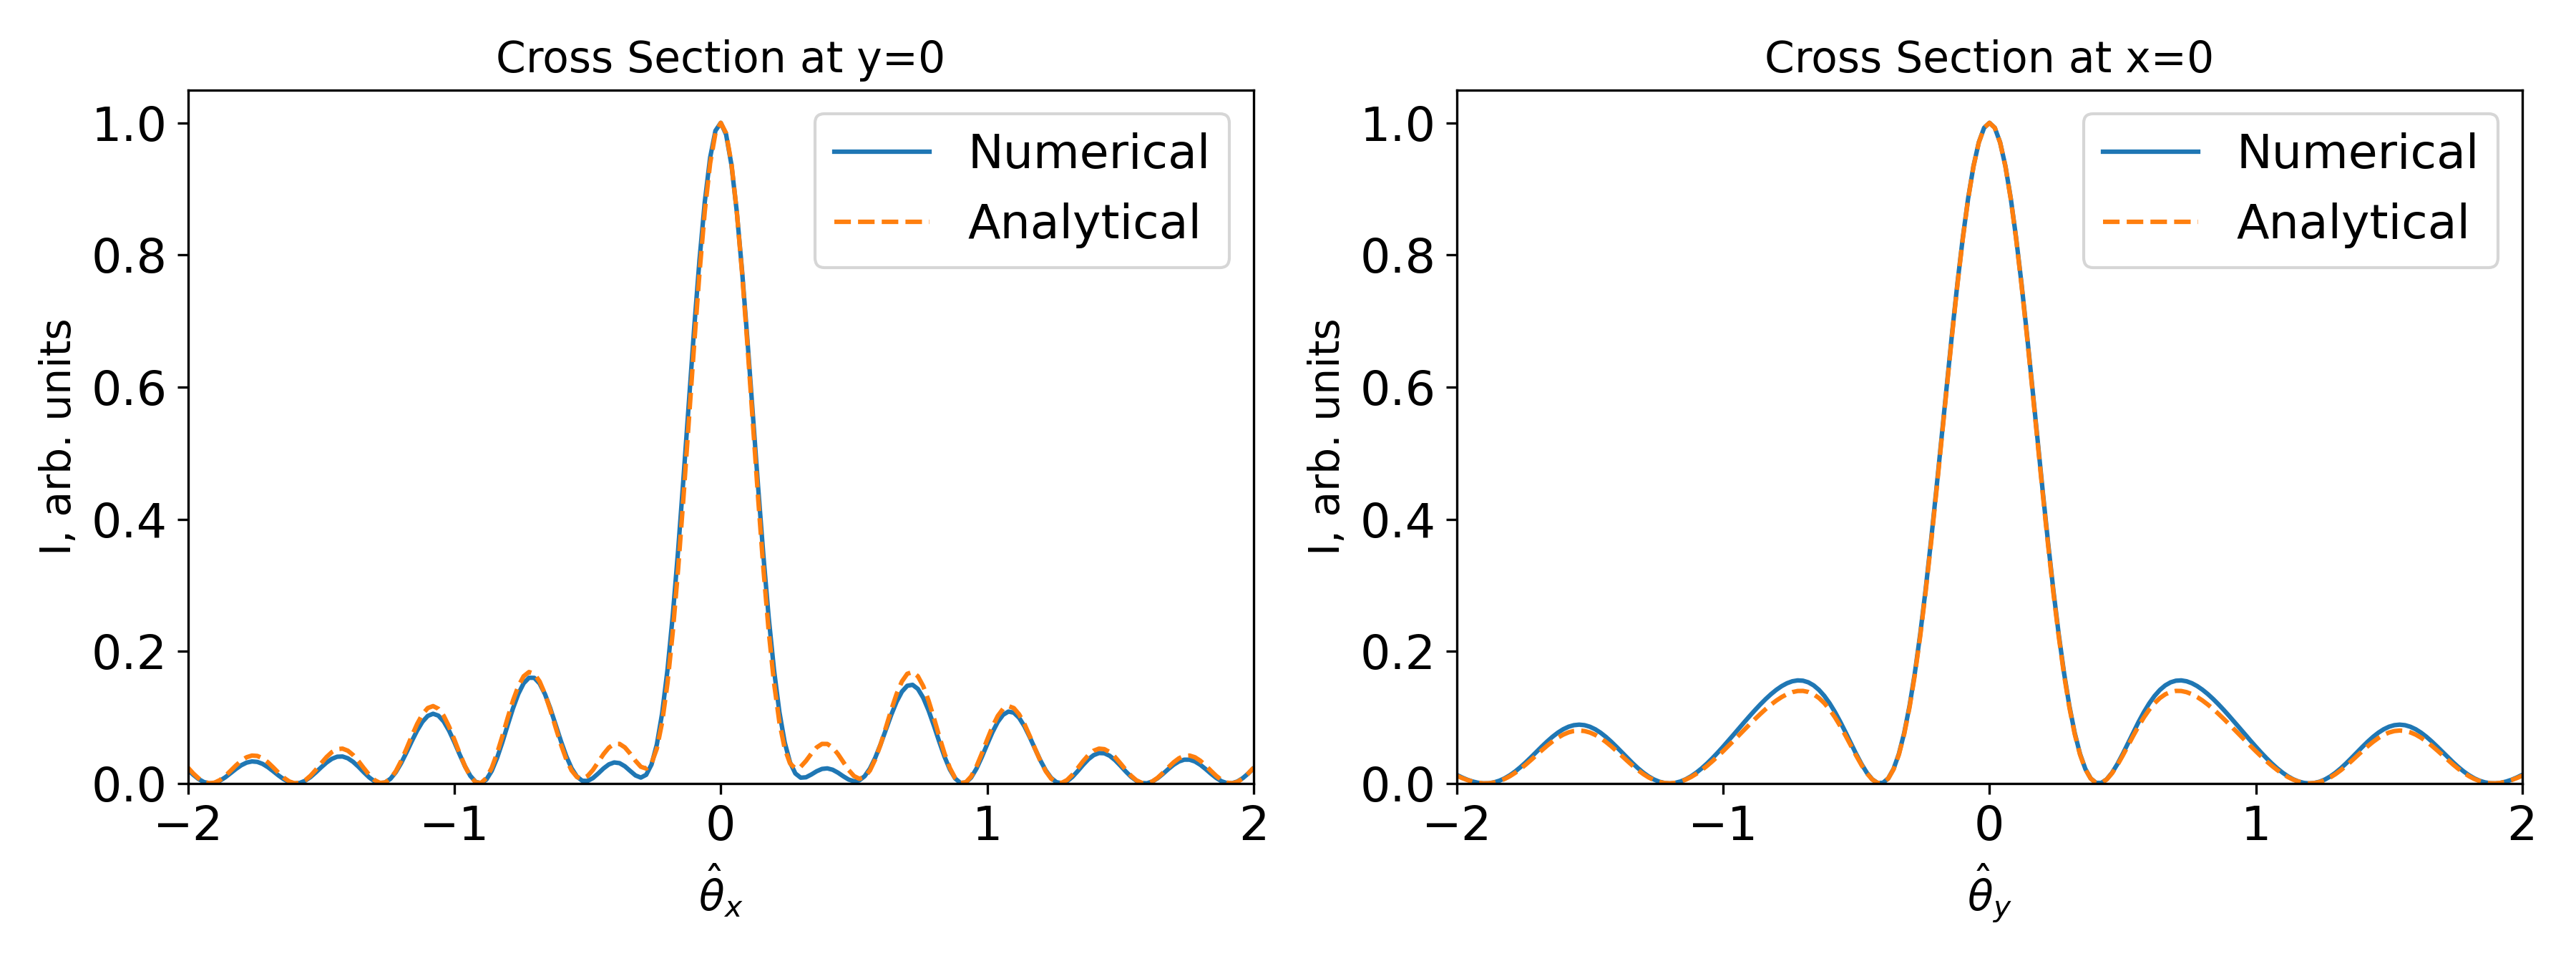
\includegraphics[width=0.99\linewidth]{content/images/5_THz_Source/pipe_check_1D.png}
        \captionsetup{justification=centering}
        \caption{Cross sections of the spatial distribution shown in Fig.~\ref{Fig:pipe_check_2D}.}
        \label{Fig:pipe_check_1D}
    \end{figure*}

    In the cross-check I show only $k=1$, other modes coincides reasonably well resulting in a more complex spatial distribution. I believe this representation is enough for a fair cross-check and more studies should be done on physical interpretation of the the computational results, which definitely should be a subject for future work.
    
\section{Discussion and outlook}
    
    The developed code is valuable for calculating insertion devices in physics situations where the influence of metallic components is substantial on the radiation. For example, this applies to applications like THz undulator sources for beamlines at FEL facilities. For these facilities, it is crucial to know the source characteristics well in order to optimize the subsequent propagation system.

    As of the moment of writing these lines (April 2024), the code has several weak points in terms of numerical efficiency. Initially written as a simple Python script to test the idea of writing the code for an arbitrary Green's function, it utilizes static memory allocation—multidimensional arrays are defined before running the code, which under certain circumstances leads to RAM overloads. Moreover, this implementation is not suitable for wrapping the code in faster programming languages like C. Numerical efficiency will need to be improved in the next releases of the code.

[[[GG ARRIVED HERE]]]